%\documentclass[xcolor={dvipsnames}]{beamer}
\documentclass[9pt]{beamer}
%\usepackage[dvipsnames]{xcolor}
%\usepackage[dvipsnames,table,xcdraw]{xcolor}

\usepackage[utf8]{inputenc}
\usepackage{caption}
\usepackage{tikz}
\usetikzlibrary{tikzmark}
\usetikzlibrary{shapes.geometric}
\usetikzlibrary{arrows,scopes} %tikz libraries used to draw the glyphs
\usetikzlibrary {3d}
\usetikzlibrary{decorations.markings}
\usepackage{circuitikz}
\usepackage{tikz-3dplot}
 \usepackage[compat=1.1.0]{tikz-feynman}
\usepackage[percent]{overpic}
\usepackage{diagbox}
\usepackage{multirow}
%\usepackage{fontspec}
\usepackage{soul}

\usepackage{hyperref}
\hypersetup{
  colorlinks=true,
  linkcolor=black,
  filecolor=magenta,      
  urlcolor=cyan,
}

\definecolor{green(ryb)}{rgb}{0.4, 0.69, 0.2}




%\usepackage{lmodern}
%\usepackage{helvet}
%\usepackage{gfsneohellenicot}
%\usepackage[light,condensed,math]{kurier}
%\usepackage[T1]{fontenc}
%\usepackage{times}
%\usepackage{tgadventor}
%\usepackage{mathpazo}
%\usepackage{palatino}
\usetheme{Boadilla}
%\usetheme{Montpellier}
%\usetheme{CambridgeUS}
%\usepackage{cmbright}
%\usepackage[OT1]{fontenc}


\usepackage[scaled]{helvet} % With " scaled " option
%\usepackage{eulervm}
%\usefonttheme[onlymath]{serif}
%\usepackage[light,math]{iwona}
%\usepackage[T1]{fontenc}

%\usepackage[sfdefault,lining]{FiraSans} %% option 'sfdefault' activates Fira Sans as the default text font
%\usepackage[fakebold]{firamath-otf}
%\renewcommand*\oldstylenums[1]{{\firaoldstyle #1}}

%\setbeamercolor*{structure}{bg=Green!20,fg=Green}

%\setbeamercolor*{palette primary}{use=structure,fg=white,bg=structure.fg}
%\setbeamercolor*{palette secondary}{use=structure,fg=white,bg=structure.fg!75}
%\setbeamercolor*{palette tertiary}{use=structure,fg=white,bg=structure.fg!50!black}
%\setbeamercolor*{palette quaternary}{fg=white,bg=black}

%\setbeamercolor{section in toc}{fg=black,bg=white}
%\setbeamercolor{alerted text}{use=structure,fg=structure.fg!50!black!80!black}

%\setbeamercolor{titlelike}{parent=palette primary,fg=structure.fg!50!black}
%\setbeamercolor{frametitle}{bg=gray!10!white,fg=PineGreen}

%\setbeamercolor*{titlelike}{parent=palette primary}



%\usetheme{Madrid}
%\usecolortheme{seahorse}
\usecolortheme{dove}
%\usecolortheme{structure}
%\usecolortheme{beetle}
%\usecolortheme{spruce}
%\usecolortheme{fly}
%\usecolortheme{dolphin}
%\usecolortheme{albatross}
%\usefonttheme{serif}

\captionsetup{font=scriptsize,labelfont=scriptsize}


\setbeamertemplate{caption}[numbered]
\setbeamertemplate{itemize item}[circle]
\setbeamertemplate{itemize subitem}[square]
\setbeamertemplate{itemize subsubitem}[triangle]

\newcommand{\backupbegin}{
  \newcounter{finalframe}
  \setcounter{finalframe}{\value{framenumber}}
}
\newcommand{\backupend}{
  \setcounter{framenumber}{\value{finalframe}}
}

%\newcommand{\pt}{$\mathnormal{p}_\mathrm{T}$ }
%\newcommand{\pthat}{$\mathnormal{\hat{p}}_\mathrm{T}$ }
\newcommand{\pt}{$p_{\text{T}}\ $}
\newcommand{\ptjet}{$p_\text{T}^\text{jet}\ $}
\newcommand{\ptmu}{$p_\text{T}^\mu\ $}
\newcommand{\pthat}{$\hat{p}_{\text{T}}\ $}

\newcommand{\rc}{%
  \resizebox{!}{1.25ex}{%
    \begin{tikzpicture}[>=round cap]
      \clip (0.09em,-0.05ex) rectangle (0.61em,0.81ex);
      \draw [line width=.11ex, <->, rounded corners=0.13ex] (0.1em,0.1ex) .. controls (0.24em,0.4ex) .. (0.35em,0.8ex) .. controls (0.29em,0.725ex) .. (0.25em,0.6ex) .. controls (0.7em,0.8ex) and (0.08em,-0.4ex) .. (0.55em,0.25ex);
    \end{tikzpicture}%
  }%
}

\tikzset{middlearrow/.style={
        decoration={markings,
            mark= at position 0.5 with {\arrow{#1}} ,
        },
        postaction={decorate}
    }
}





%Information to be included in the title page:
\title[Thesis Preliminary Exam] %optional
      {\textbf{Thesis Preliminary Exam}}

\author[Clayton Bennett] % (optional, for multiple authors)
       {Clayton Bennett}

\institute[UIC] % (optional)
{
               
  University of Illinois at Chicago \\
  The CMS Collaboration
  
}

\date[4 Dec 2023] % (optional)
     {December 4, 2023}


     \begin{document}
     \graphicspath{ {/home/clayton/Documents/nuclear/GroupMeeting/figures} }

     \begin{frame}
       \titlepage
       \begin{columns}
	 \column{0.2\textwidth}
	 \centering
	 \begin{figure}
	   \includegraphics[width=0.8\textwidth]{CMSlogo}
	 \end{figure}
	 \column{0.6\textwidth}
	 
	 \column{0.2\textwidth}
	 \begin{figure}
	   \includegraphics[width=0.8\textwidth]{UIClogo}
	 \end{figure}
       \end{columns}
     \end{frame}

     \graphicspath{ {/home/clayton/Documents/nuclear/thesisPrelim/figures} }



     \begin{frame}
  \frametitle{\textbf{Outline}}
  \begin{enumerate}
  \item \label{th1} The Quark Gluon Plasma
  \item \label{th2} Jets as probes of the Quark Gluon Plasma
  \item \label{th3} $b$-jet measurements with CMS
  \end{enumerate}

  \

  \begin{columns}
    \column{0.4\textwidth}
    \begin{tikzpicture}
      \node{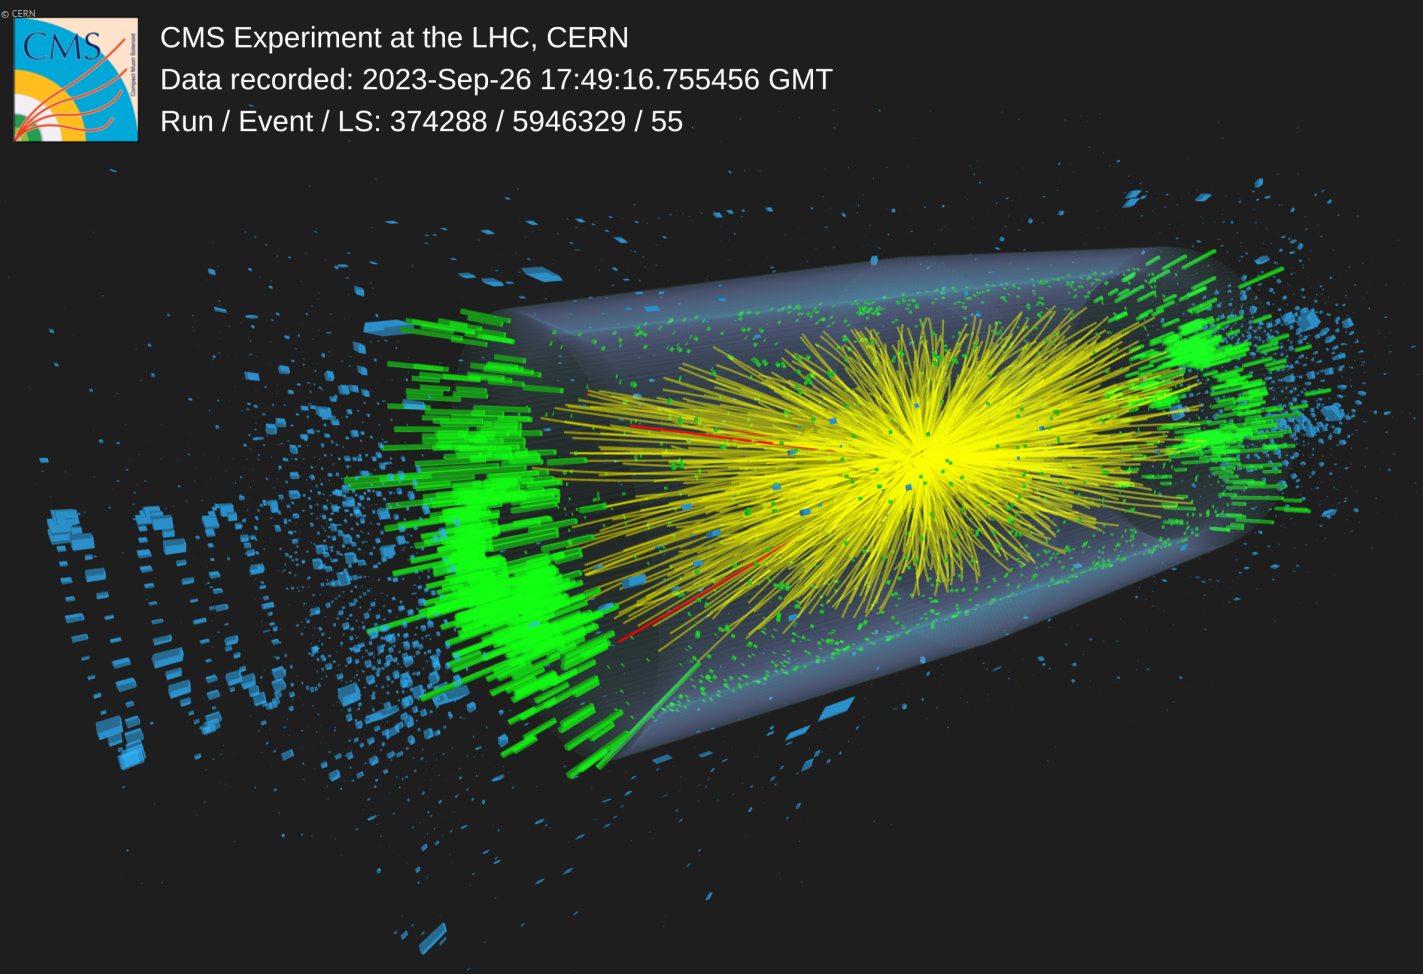
\includegraphics[width=\textwidth]{event-display-1.png}};
    \end{tikzpicture}
    \column{0.4\textwidth}
    \begin{tikzpicture}
      \node{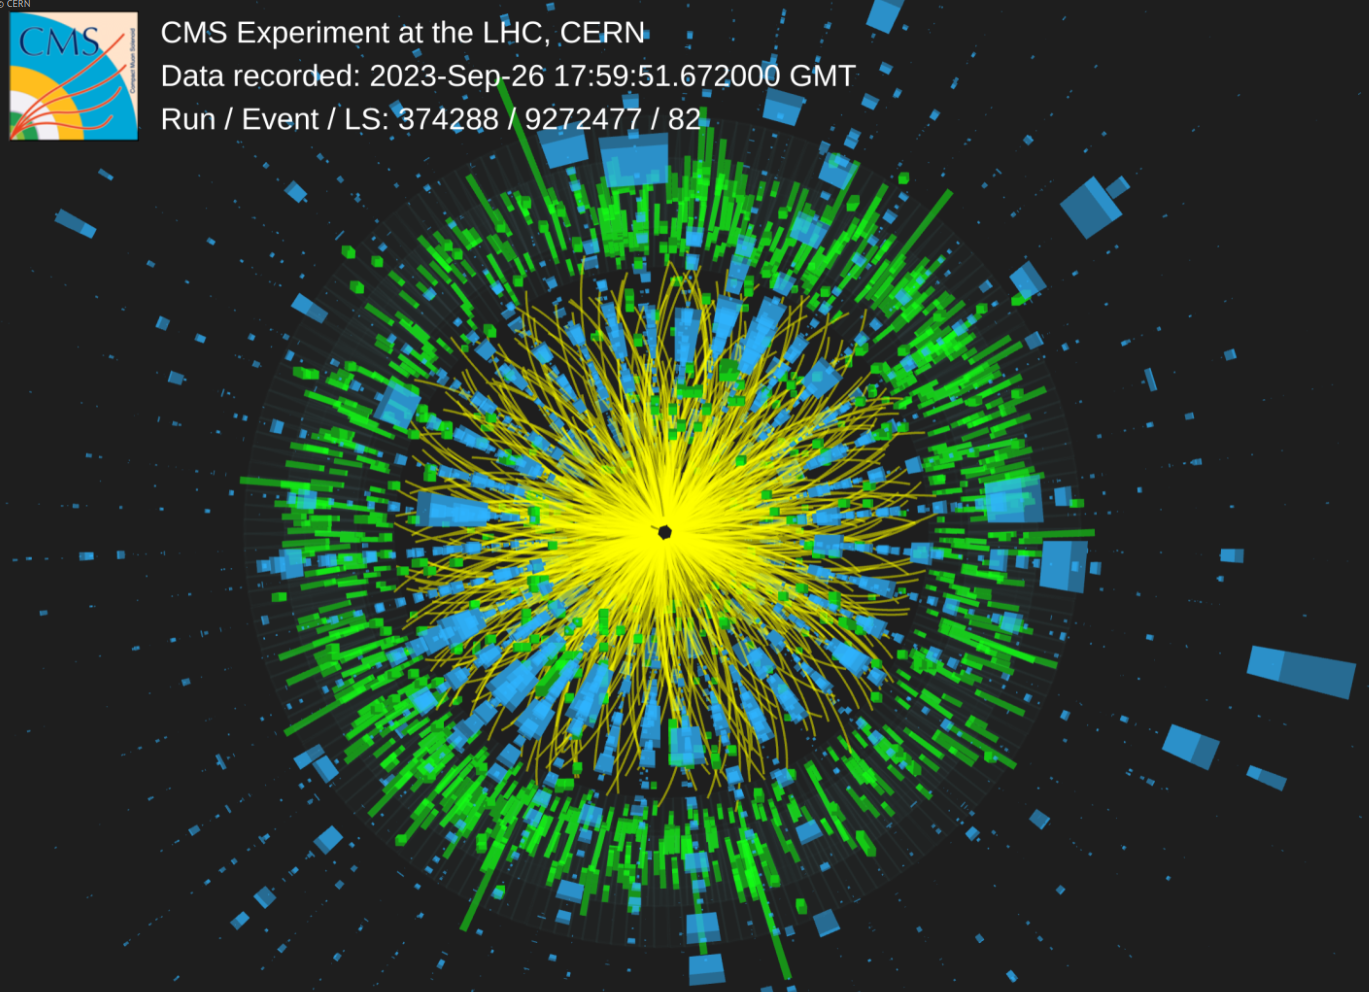
\includegraphics[width=\textwidth]{event-display-2.png}};
    \end{tikzpicture}
  \end{columns}
  \centering \scriptsize First 2023 PbPb collision at 5.36 TeV
\end{frame}

     \begin{frame}
  \centering \textbf{The Quark Gluon Plasma}
\end{frame}

     \begin{frame}
  \frametitle{\textbf{The Standard Model of Particle Physics}}
  \begin{columns}
    \column{0.65\textwidth}
    \begin{tikzpicture}
      \node{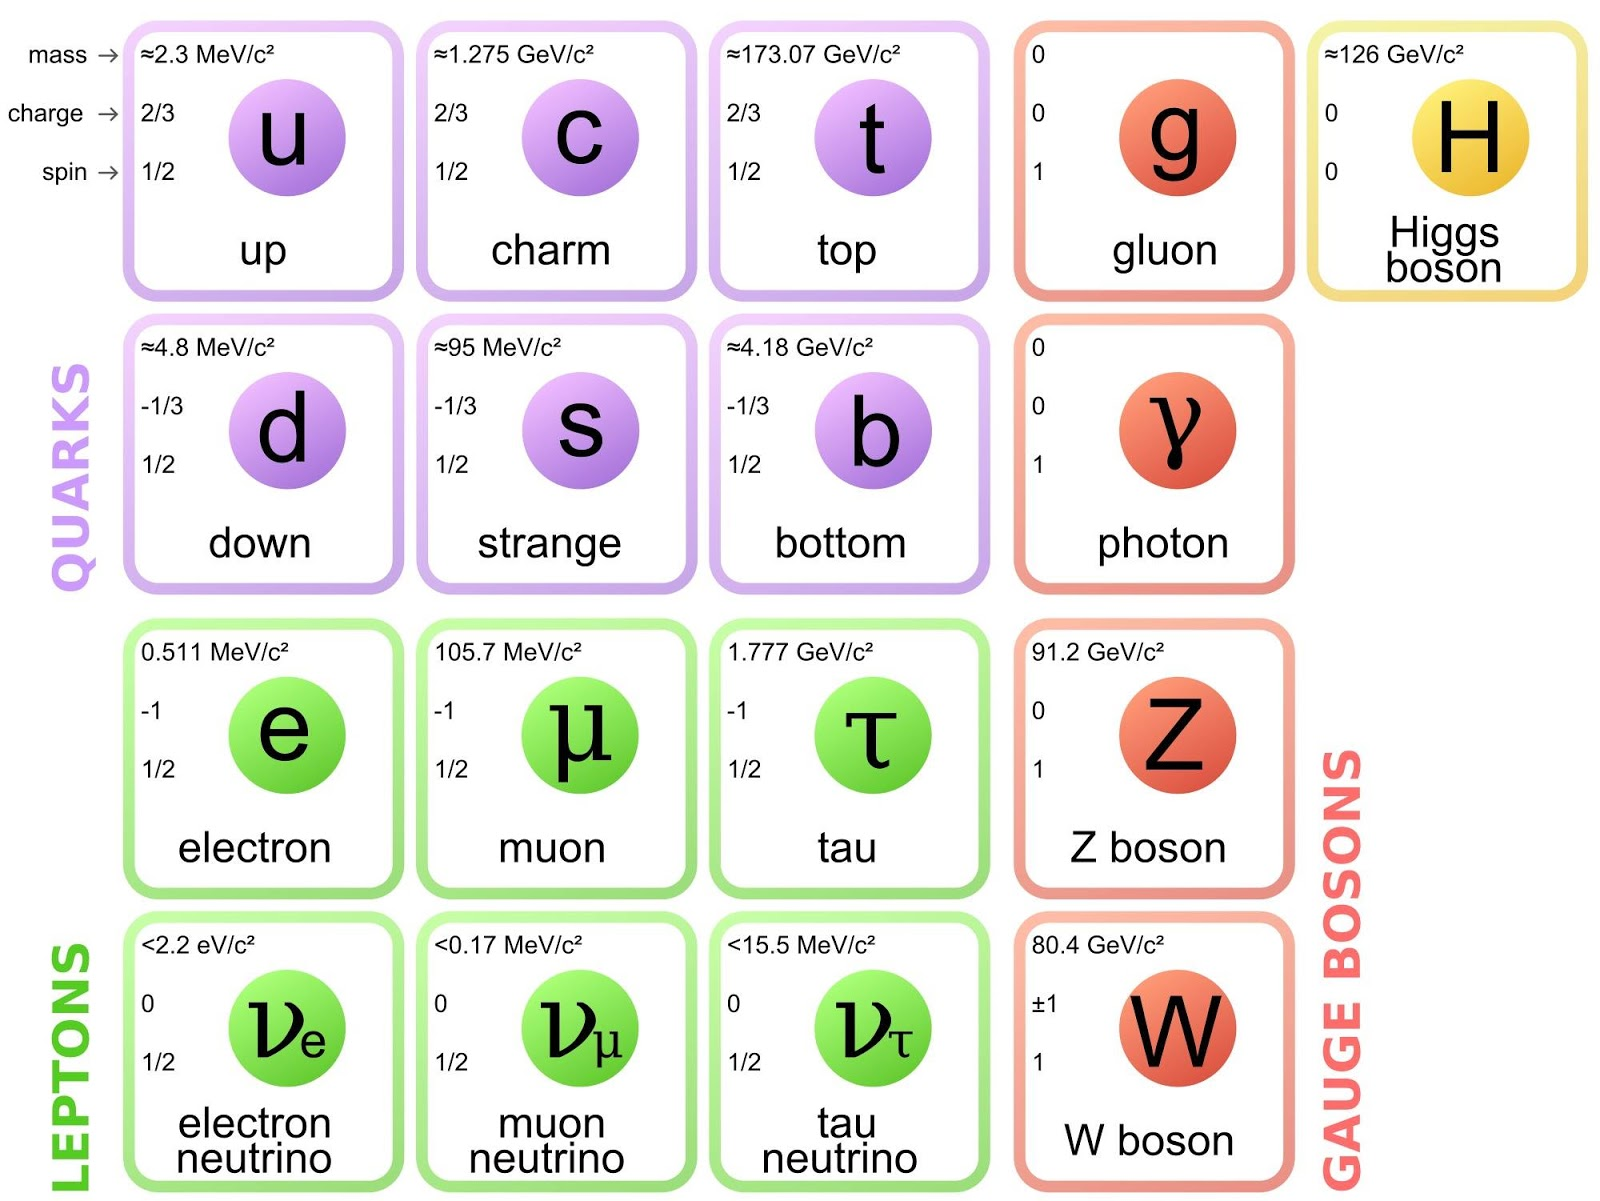
\includegraphics[width=\textwidth]{standard-model.jpg}};
      \node[font=\tiny] at (-1.5,-3.2) {\href{https://en.wikipedia.org/wiki/Standard_Model}{https://en.wikipedia.org/wiki/Standard\_Model}};
    \end{tikzpicture}
    \column{0.35\textwidth}
    \begin{itemize}
    \item Quantum field theory that describes
      \begin{itemize}
      \item Quantum electrodynamics
      \item Electroweak interactions
      \item Quantum chromodynamics
      \item \st{Gravity}
      \end{itemize}
    \item Quarks and leptons interact via the exchange of gauge bosons
      \begin{itemize}
      \item QED $\to \gamma$
      \item EW $\to W^{\pm}, Z$
      \item QCD $\to g$
      \end{itemize}
    \item $H$ is a mass-giving scalar boson
    \item \textbf{Experimentally verified}
    \item Still open questions...
      \begin{itemize}
      \item muon $g-2$ anomaly
      \item non-zero neutrino mass
      \item baryon asymmetry
      \end{itemize}
    \end{itemize}
  \end{columns}
\end{frame}


     \begin{frame}
  \frametitle{\textbf{Quantum Chromodynamics}}
  \begin{columns}
    \column{0.6\textwidth}
    \begin{itemize}
    \item \textbf{Quantum chromodynamics} (QCD) is a quantum field theory describing the \textbf{strong interaction} between \textbf{quarks} and \textbf{gluons}
    \item \textbf{Confinement}: fundamental feature of QCD
      \begin{align*}
        V_{\text{QCD}}(Q^2) = \color{gray}\underbrace{\color{black}-\cfrac{4}{3}\cfrac{\alpha_s(Q^2)}{r}}_{\text{QED-like short-range}} \color{black} + \color{gray} \underbrace{\color{black}\lambda r}_{\text{QCD long-range}}
      \end{align*}
    \item QCD is a quantum field theory with \textbf{asymptotic freedom}
    \end{itemize}
    \begin{align*}
      &\alpha_s(Q^2) = \cfrac{\alpha_s(\mu^2)}{1 + \left[\alpha_s(\mu^2)\frac{(11n_c - 2n_f)}{12\pi}\right]\ln\left(\frac{Q^2}{\mu^2}\right)} \\
      & \boxed{\lim_{Q \to \infty}\alpha_s(Q^2) \to 0}
    \end{align*}

    \begin{itemize}
    \item Large $Q^2 \to$ strong-force coupling gets \textbf{weaker}
    \end{itemize}



    \column{0.4\textwidth}
    \centering
    \begin{tikzpicture}
      \node{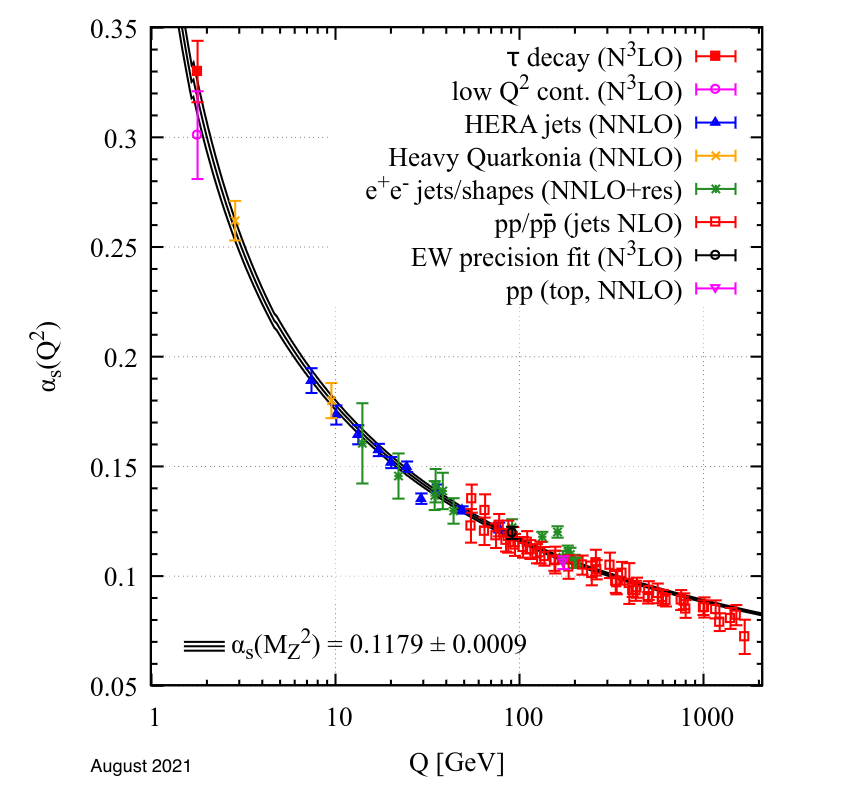
\includegraphics[width=0.9\textwidth]{running-coupling.png}};
      \node[font=\tiny,align=left] at (0.2,2.1) {\href{https://academic.oup.com/ptep/article/2022/8/083C01/6651666}{Prog. Theor. Exp. Phys. 2022, 083C01 (2022)}};
    \end{tikzpicture}

    \

    \

    \begin{columns}

      \column{0.33\textwidth}
      \resizebox{\textwidth}{\textwidth}{
        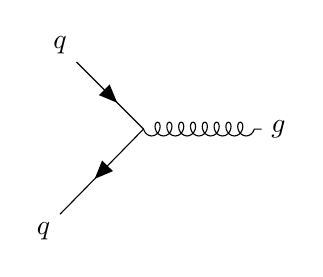
\begin{tikzpicture}
          \begin{feynman}
            \vertex (a) {\( q \)};
            \vertex[below right=of a] (b);
            \vertex[below left=of b] (c) {\( q \)};
            \vertex[right=of b] (d) {\( g \)};
            \diagram*{
              (a) -- [fermion] (b),
              (b) -- [fermion] (c),
              (b) -- [gluon] (d),
            };
          \end{feynman}
        \end{tikzpicture}
      }

      \column{0.33\textwidth}
      \resizebox{\textwidth}{\textwidth}{
        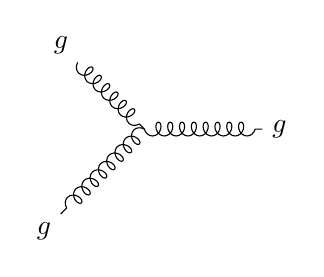
\begin{tikzpicture}
          \begin{feynman}
            \vertex (a) {\( g \)};
            \vertex[below right=of a] (b) ;
            \vertex[below left=of b] (c) {\( g \)};
            \vertex[right=of b] (d) {\( g \)};
            \diagram*{
              (a) -- [gluon] (b),
              (b) -- [gluon] (c),
              (b) -- [gluon] (d),
            };
          \end{feynman}
        \end{tikzpicture}
      }

      \column{0.33\textwidth}
      \resizebox{\textwidth}{\textwidth}{
        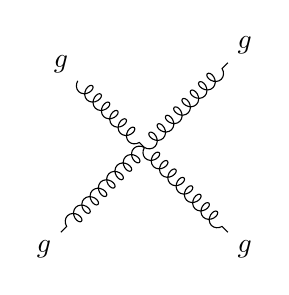
\begin{tikzpicture}
          \begin{feynman}
            \vertex (a) {\( g \)};
            \vertex[below right=of a] (b) ;
            \vertex[below left=of b] (c) {\( g \)};
            \vertex[above right=of b] (d) {\( g \)};
            \vertex[below right=of b] (e) {\( g \)};
            \diagram*{
              (a) -- [gluon] (b),
              (b) -- [gluon] (c),
              (b) -- [gluon] (d),
              (b) -- [gluon] (e),
            };
          \end{feynman}
        \end{tikzpicture}
      }

    \end{columns}
    

    
  \end{columns}
\end{frame}

     \begin{frame}
  \frametitle{\textbf{Deconfinement in heavy-ion collisions}}
  \begin{columns}
    \column{0.5\textwidth}
    \begin{itemize}
    %\item Discretize spacetime to lattice and simulate quark-gluon interactions $\to$ ``lattice QCD''
    \item Lattice QCD predicts that partons break away from strong-force bonds at sufficent energy density $\to$ \textbf{deconfinement}
    \end{itemize}
    \begin{itemize}
    \item Critical temperature ($T_c$)
      \begin{itemize}
      \item $T_c$ via lattice QCD / simple confinement models ($\mu_B = 0$)
      \item $T_c$ for non-zero $\mu_B$ is challenging
      \item state-of-the-art: $\boldmath{T_c \approx 158.0 \pm 0.6 \textbf{ MeV}}$
      \end{itemize}
    \item Evidence of $T_{\text{exp}} > T_c$
      \begin{itemize} 
      \item Estimations of particle ratios
        \begin{itemize}
        \item $dn_i \sim \exp\left\{ (E_i - \mu_B) / T  \right\} d^3 p_i$
        \item $\cfrac{\bar{p}}{p} = \exp\left\{-2\mu_B / T \right\}$
        \item $\cfrac{K}{\pi} = \exp\left\{-(E_K - E_\pi)/T  \right\}$
        \end{itemize}
      
   
      
      \end{itemize}

      \item System at extreme $T$ and $P$ $\to$ deconfined phase of quarks and gluons $\to$ \textbf{Quark Gluon Plasma} (QGP)

      %\item Statistical thermodynamics in QCD $\to$ $m_{\pi} \lesssim$ 140 MeV (1965)
    %\item Lattice QCD (at $\mu_B \sim 0$) $\to$ $T_C \approx 
    %\item Lattice QCD predicts a deconfined phase of quarks and gluons known as the \textbf{Quark Gluon Plasma} at extreme temperatures and pressures
    %\item At $\mu_B \sim 0$, the critical temperature for this phase-change is $\boldmath{T_c \approx 158.0 \pm 0.6 \textbf{ MeV} \approx 1.8 \cdot 10^{12} \textbf{ K}}$
    \end{itemize}
    \column{0.5\textwidth}
    \centering 
    \begin{tikzpicture}
      \node{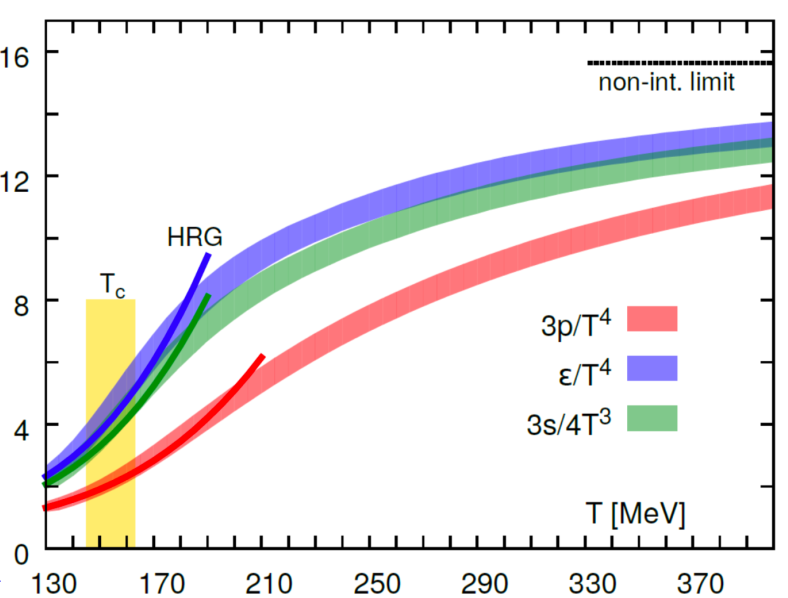
\includegraphics[width=0.8\textwidth]{qcd-phase-change-alt.png}};
      \node[font=\tiny,align=left] at (1.2,2.0) {\textbf{Lattice QCD phase change}};
      \node[font=\scriptsize,align=left] at (-1,1.5) {$\boldmath{\mu_B = 0}$};
      \node[font=\scriptsize,align=left,rotate=90] at (-2.6,0.7) {Degrees of freedom};
      %\node[font=\tiny,align=left] at (1.2,1.6) {\href{https://doi.org/10.1016/j.physletb.2019.07.014}{https://doi.org/10.1016/j.physletb.2019.07.014}};
    \end{tikzpicture}

    \

    \begin{tikzpicture}
      \node{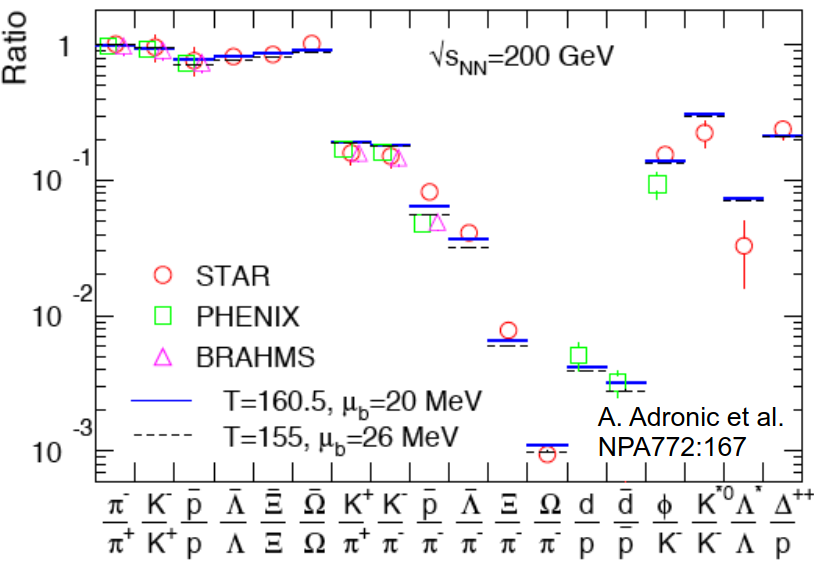
\includegraphics[width=0.8\textwidth]{particle-ratios.png}};
      \node[font=\tiny,align=left] at (1.2,1.85) {\textbf{Particle ratios at RHIC}};
    \end{tikzpicture}
%    \begin{tikzpicture}
%      \node{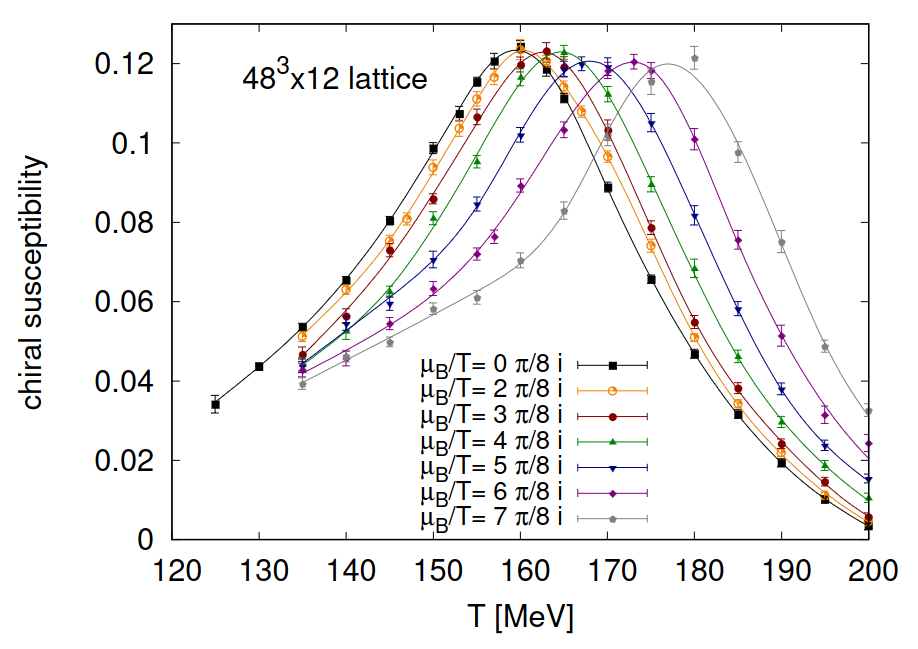
\includegraphics[width=0.9\textwidth]{chiral-susceptibility.png}};
%      \node[font=\tiny,align=left] at (1.2,1.6) {\href{https://arxiv.org/abs/2002.02821}{arXiv:2002.02821}};
%    \end{tikzpicture}
  \end{columns}
\end{frame}

     \begin{frame}
  \frametitle{\textbf{Phases of QCD}}
  \begin{itemize}
  \item For $\mathbf{\frac{\mu_B}{T} \leq 2}$, QGP-to-hadron phase transition is a \textbf{smooth crossover}
  \item Above some critical point, the QGP-to-hadron transition is expected to become a \textbf{first-order phase transition}
  \end{itemize}

  \

  \centering
  \begin{tikzpicture}
    \node{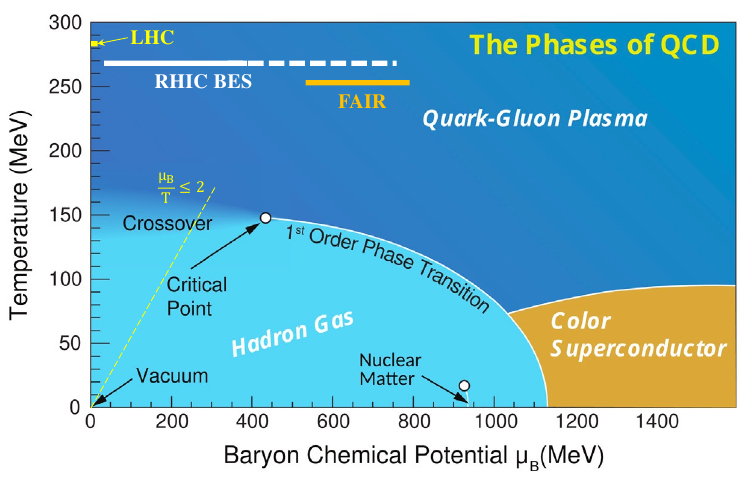
\includegraphics[width=0.8\textwidth]{qcd-phase-diagram.png}};
    \node[font=\tiny,align=left] at (3.5,3) {\href{https://arxiv.org/abs/2303.17254}{arXiv:2303.17254}};
  \end{tikzpicture}
\end{frame}

     \begin{frame}
  \frametitle{\textbf{QGP at Particle Colliders}}
  \begin{itemize}
  \item We can create QGP in the lab by colliding heavy nuclei ($v \approx c$) in particle accelerators (such as RHIC and LHC)
  \item QCD predicts rich phase dynamics prior to particle detection
    \begin{itemize}
    \item Non-equilibrated initial state
    \item \textbf{Strongly-interacting QGP phase} that flows as a relativistic hydrodynamic fluid
    \item Medium expansion, cooling, and \textbf{hadronization}
    \item Hadronic rescattering and \textbf{freeze-out}
    \end{itemize}
  \end{itemize}

  \
  
  \centering
  \begin{tikzpicture}
    \node{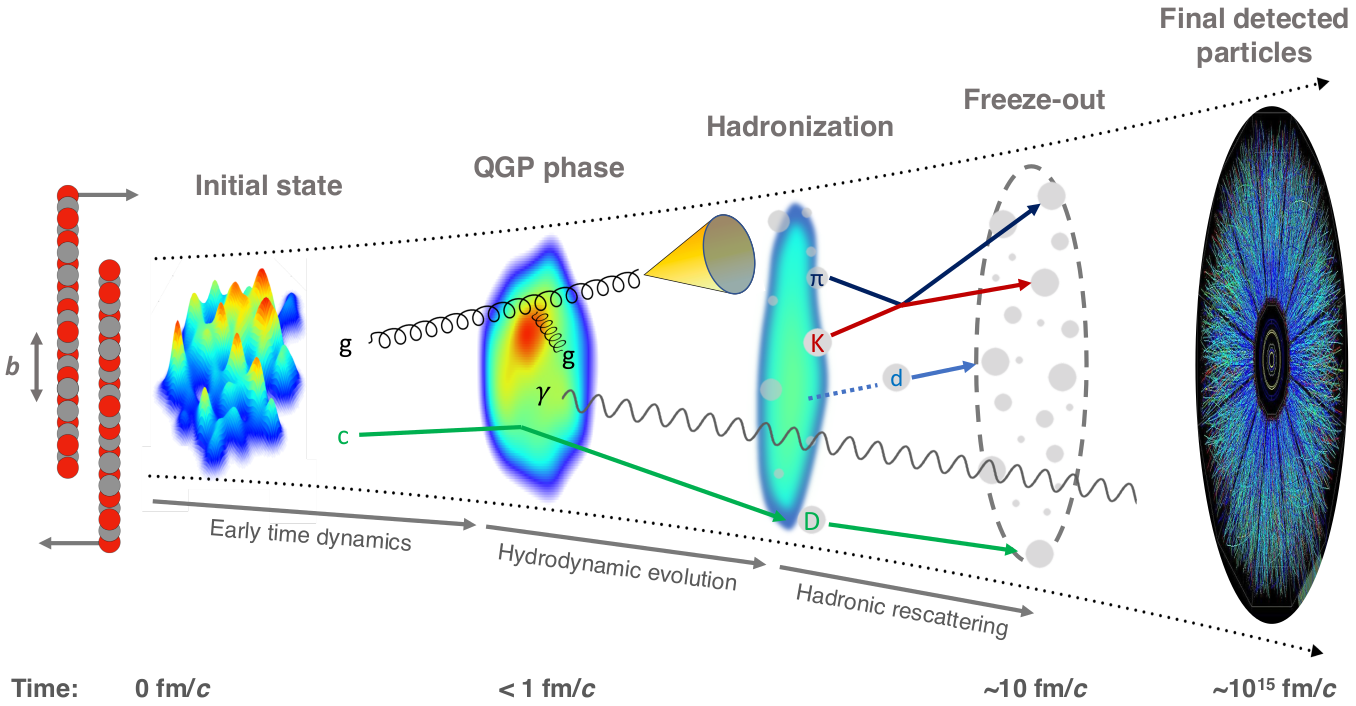
\includegraphics[width=0.8\textwidth]{collision-stages.png}};
  \end{tikzpicture}
\end{frame}

     \begin{frame}
  \frametitle{\textbf{Kinematics}}
  \begin{columns}
    \column{0.4\textwidth}
    \centering
    \newcommand \px {0.6}
    \newcommand \py {1.3}
    \newcommand \pz {0.8}
    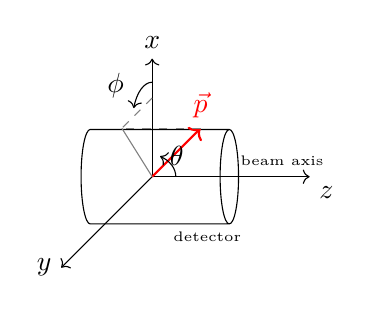
\begin{tikzpicture}
      \tdplotsetmaincoords{70}{110}
      \draw[->] (0,0,0) to (xyz cylindrical cs:radius=2) node[anchor=north west]{$z$};
      \draw[->] (0,0,0) to (xyz cylindrical cs:radius=1.5,angle=90) node[anchor=south]{$x$};
      \draw[->] (0,0,0) to (xyz cylindrical cs:z=3) node[anchor=east]{$y$};
      \node[cylinder, draw, shape aspect=1, minimum height = 2cm, minimum width = 1.2cm] {};
      \draw[->,color=red,thick] (0,0,0) to (\px,\py,\pz) node[color=red,thick,anchor=south]{$\vec{p}$};
      \draw[-,color=gray] (0,0,0) to (0.0,\py,\pz);
      %\draw[-,color=gray] (0,0,0) to (\px,\py,0.0);
      %\draw[-,dashed,color=gray] (\px,\py,\pz) to (\px,\py,0.0);
      \draw[-,dashed,color=gray] (\px,\py,\pz) to (0.0,\py,\pz);
      \draw[-,dashed,color=gray] (0.0,\py,0.0) to (0.0,\py,\pz);
      %\draw[-,dashed,color=gray] (0.0,\py,0.0) to (\px,\py,0.0);
      \draw[->] (.3,0,0) arc [start angle=0,end angle=60,x radius=0.4,y radius=0.3] node[anchor=west]{$\text{  }\theta$};
      \draw[->] (0,1.2,0) arc [start angle=90,end angle=160,x radius=0.25,y radius=0.5] node[anchor=south east]{\ $\phi$};
      \node[font=\tiny] at (0.7,-0.76) {detector};
      \node[font=\tiny] at (1.65,0.2) {beam axis};
    \end{tikzpicture}
    \column{0.6\textwidth}
    \begin{itemize}
    \item Detector geometry warrants the use of cylindrical coordinate system
    \end{itemize}
    \begin{align*}
      \text{transverse momentum} : p_{\text{T}} &= \left|\vec{p}\right| \sin\theta \\
      \text{rapidity} : y &= \cfrac{1}{2} \ln \left( \cfrac{E + p_z}{E - p_z} \right)
      \\
      \text{psuedo-rapidity} :\eta &= \cfrac{1}{2} \ln \left( \cfrac{p + p_z}{p - p_z} \right) \\
      & \to -\ln \left[ \tan\left(\cfrac{\theta}{2}\right) \right]
    \end{align*}
    \begin{itemize}
    \item Why are these variables common in particle physics experiments?
      \begin{itemize}
      \item $\sum_{i} p_{\text{T},i} = 0 + \epsilon$
      \item $y$ is invariant for boosts along $z$-axis
      \end{itemize}
    \end{itemize}
  \end{columns}
  
  
\end{frame}

     \begin{frame}
  \frametitle{\textbf{Centrality}}
\end{frame}

     \begin{frame}
  \frametitle{\textbf{Flow in HI Collisions}}
  \begin{columns}
    \column{0.5\textwidth}
    \begin{itemize}
    \item QGP is often modeled as a \textbf{hydrodynamic fluid} $\to$ initial spacial anisotropies result in momentum-space anisotropies
    \item Flow harmonics $v_n$ $\to$ quantify the $\phi$-space anisotropy
    \end{itemize}
    \begin{align*}
      \cfrac{dN}{d\phi} = A \cdot \left( 1 + 2\sum_{n = 1}^{\infty} v_n \cos\left[n(\phi - \bar{\Psi}_{n})\right]   \right) 
    \end{align*}
    \begin{itemize}
    \item $v_2$ is most closely correlated with the initial-state geometry
    \item $v_2$ scales with parton number $\to$ flow is contributed on the parton level   $\to$ \textbf{evidence of deconfinement}
    \item Hydrodynamic models $\to$ QGP is a near \textit{perfect fluid}
    \end{itemize}
    \column{0.4\textwidth}
    \only<1>{
      \centering
      
      \begin{tikzpicture}
        \node{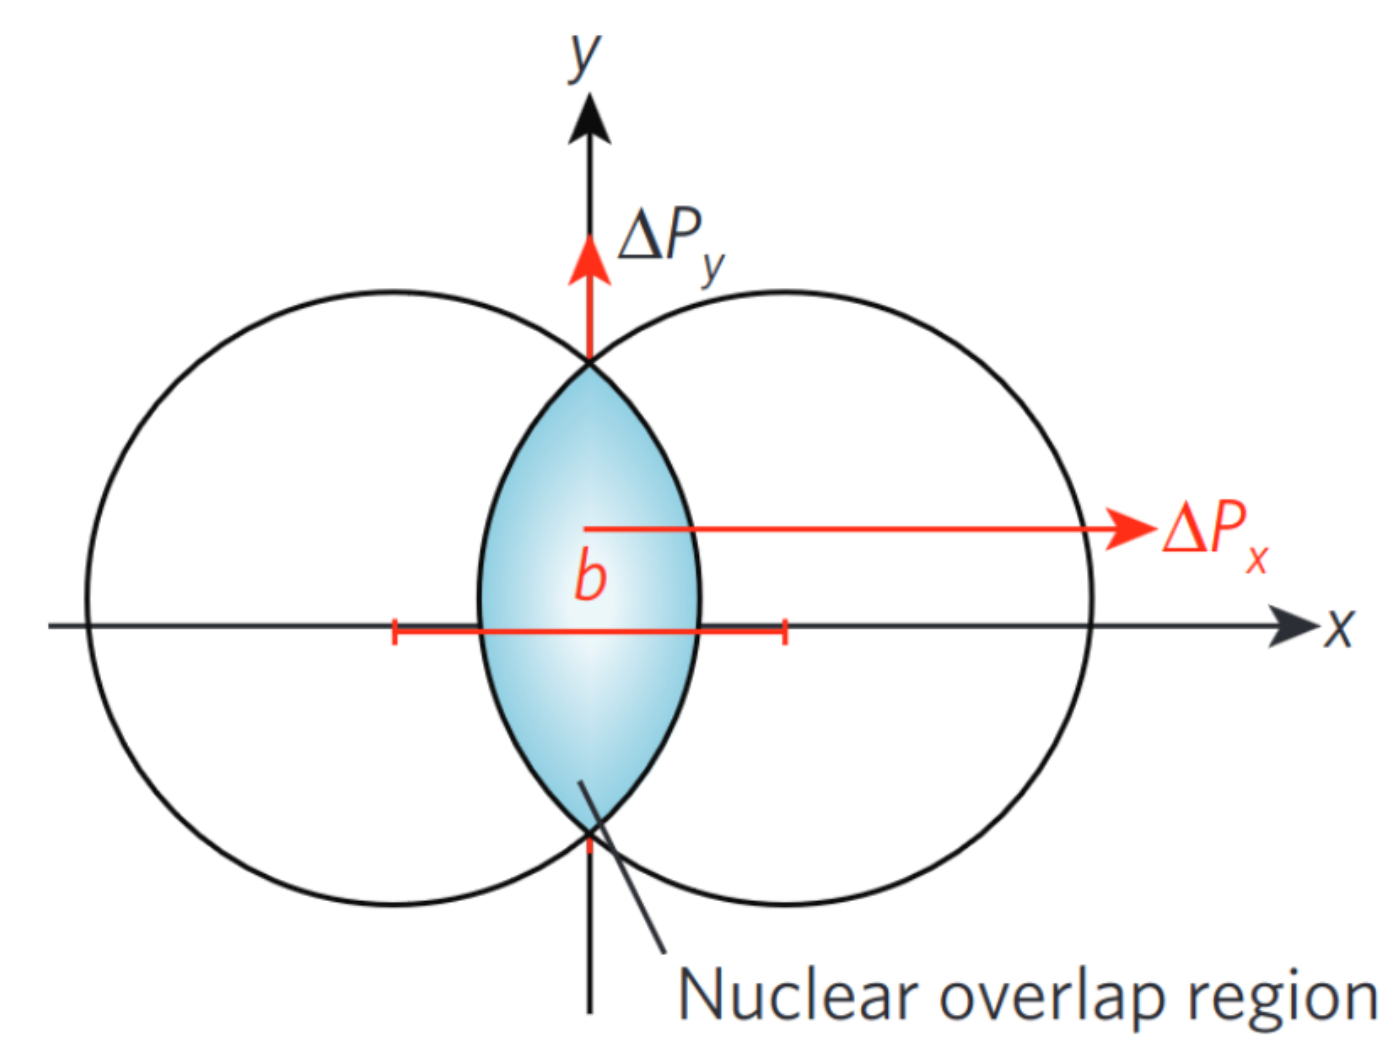
\includegraphics[width=0.8\textwidth]{nuclear-overlap-region-crop.png}};
      \end{tikzpicture}

      \
      
      \begin{tikzpicture}
        \node{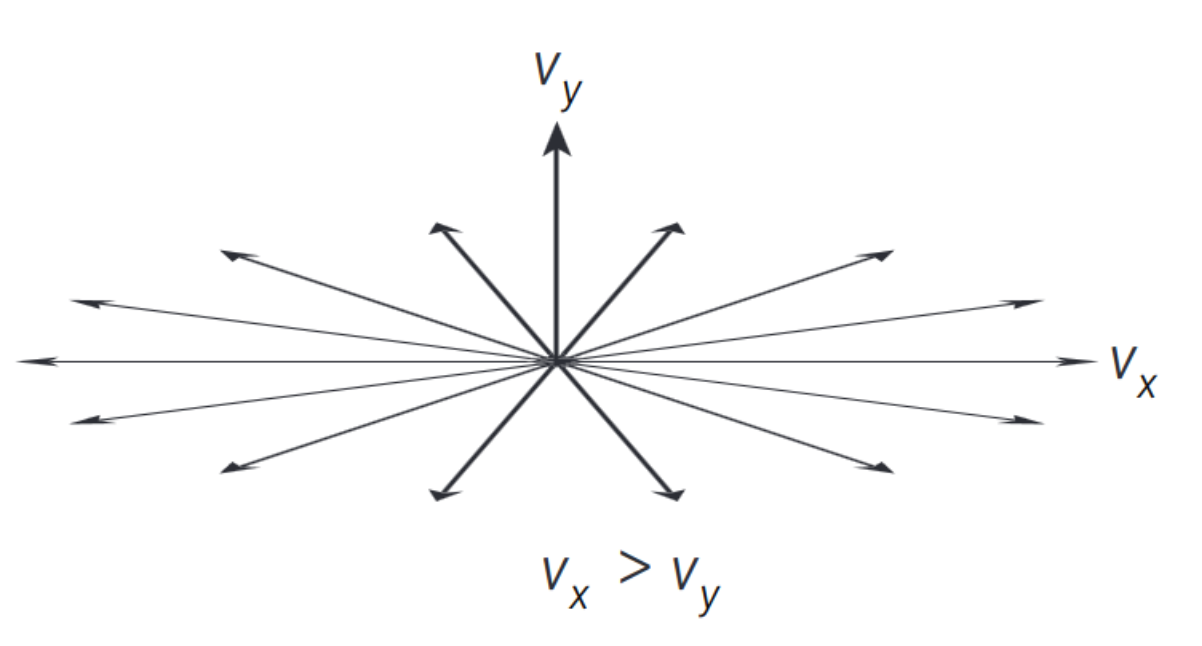
\includegraphics[width=0.8\textwidth]{velocity-anisotropy.png}};
        \node[font=\tiny] at (1.5,-1) {\href{https://arxiv.org/abs/1802.04801}{arXiv:1802.04801}};
      \end{tikzpicture}

      \

      
      \begin{tikzpicture}
        \node{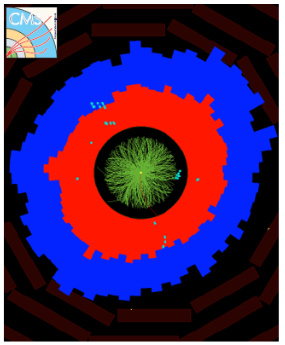
\includegraphics[width=0.35\textwidth]{asymmetric-event-display.png}};
      \end{tikzpicture}
      \begin{tikzpicture}
        \node{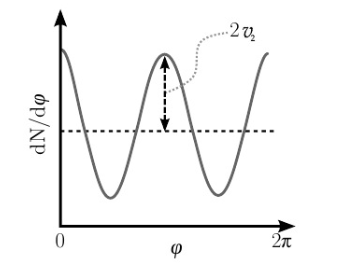
\includegraphics[width=0.5\textwidth]{dn-dphi.png}};
      \end{tikzpicture}

      
    }

    \only<2>{
      \centering
      \begin{tikzpicture}
        \node{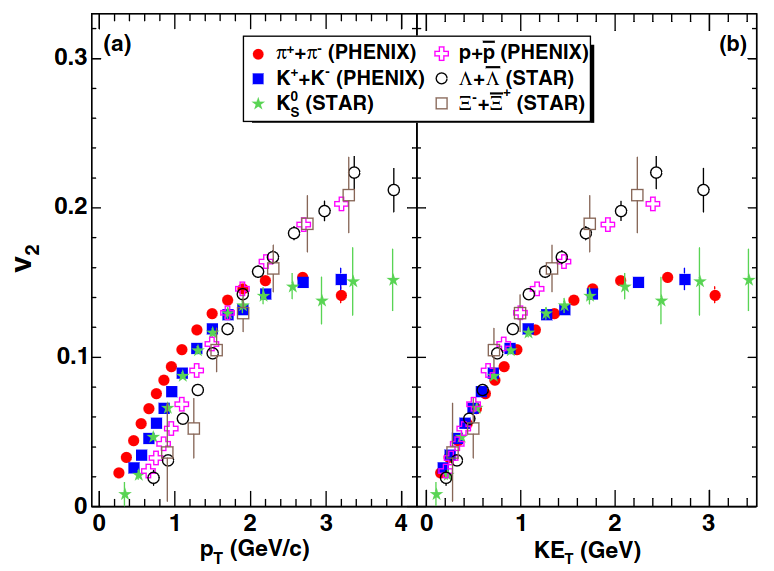
\includegraphics[width=\textwidth]{v2-before-scaling.png}};
        \node[font=\tiny,align=left] at (-1,0.5) {\textbf{baryons}};
        \node[font=\tiny,align=left] at (-0.3,-0.4) {\textbf{mesons}};
        \node[font=\tiny,align=left] at (1.0,0.5) {\textbf{baryons}};
        \node[font=\tiny,align=left] at (1.7,-0.4) {\textbf{mesons}};
        \node[font=\tiny] at (1.3,1.9) {\href{https://journals.aps.org/prl/abstract/10.1103/PhysRevLett.98.162301}{Phys. Rev. Lett. 98, 162301}};
      \end{tikzpicture}

      \
      
      \begin{tikzpicture}
        \node{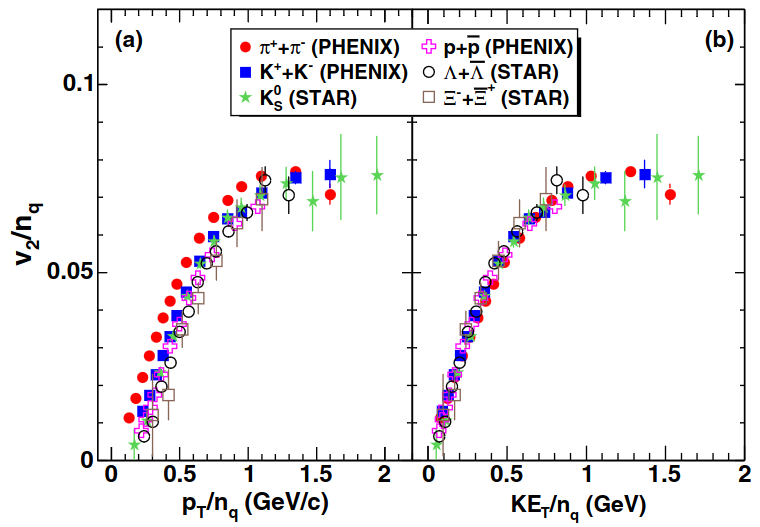
\includegraphics[width=\textwidth]{v2-after-scaling.png}};
      \end{tikzpicture}
      
    }
    

    
  \end{columns}
    
\end{frame}

     \begin{frame}
  \frametitle{\textbf{Strangeness Enhancement in HI Collisions}}

  \begin{columns}
    

    \column{0.5\textwidth}
    \centering
    \begin{itemize}
    \item QGP state $\to$ increased production of $s$ and $\bar{s}$ quarks
    \item Expect an yield-increase in strange particles
      \begin{itemize}
      \item $\Lambda(uds)$, $\bar{\Lambda}(\bar{u}\bar{d}\bar{s})$
      \item $\Xi(dss)$, $\bar{\Xi}(\bar{d}\bar{s}\bar{s})$
      \item $\Omega(sss)$, $\bar{\Omega}(\bar{s}\bar{s}\bar{s})$
      \end{itemize}
    \item Enhancement increases with strangeness and multiplicity $\to$ \textbf{consistent with QGP formation}
    \end{itemize}

    \column{0.5\textwidth}
    \centering
    \begin{tikzpicture}
      \node{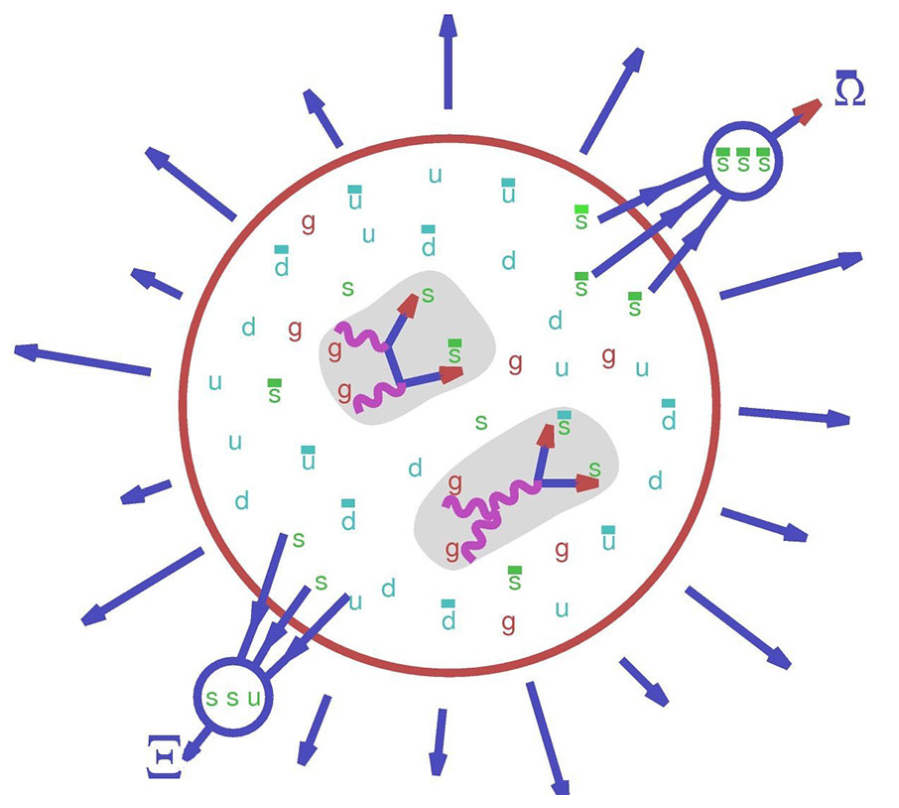
\includegraphics[width=0.7\textwidth]{strangeness-production.png}};
      \node[font=\tiny] at (1.8,-1.7) {\href{https://link.springer.com/article/10.1140/epja/i2015-15114-0}{Eur. Phys. J. A (2015) 51: 114}};
    \end{tikzpicture}

    \

    \begin{tikzpicture}
      \node{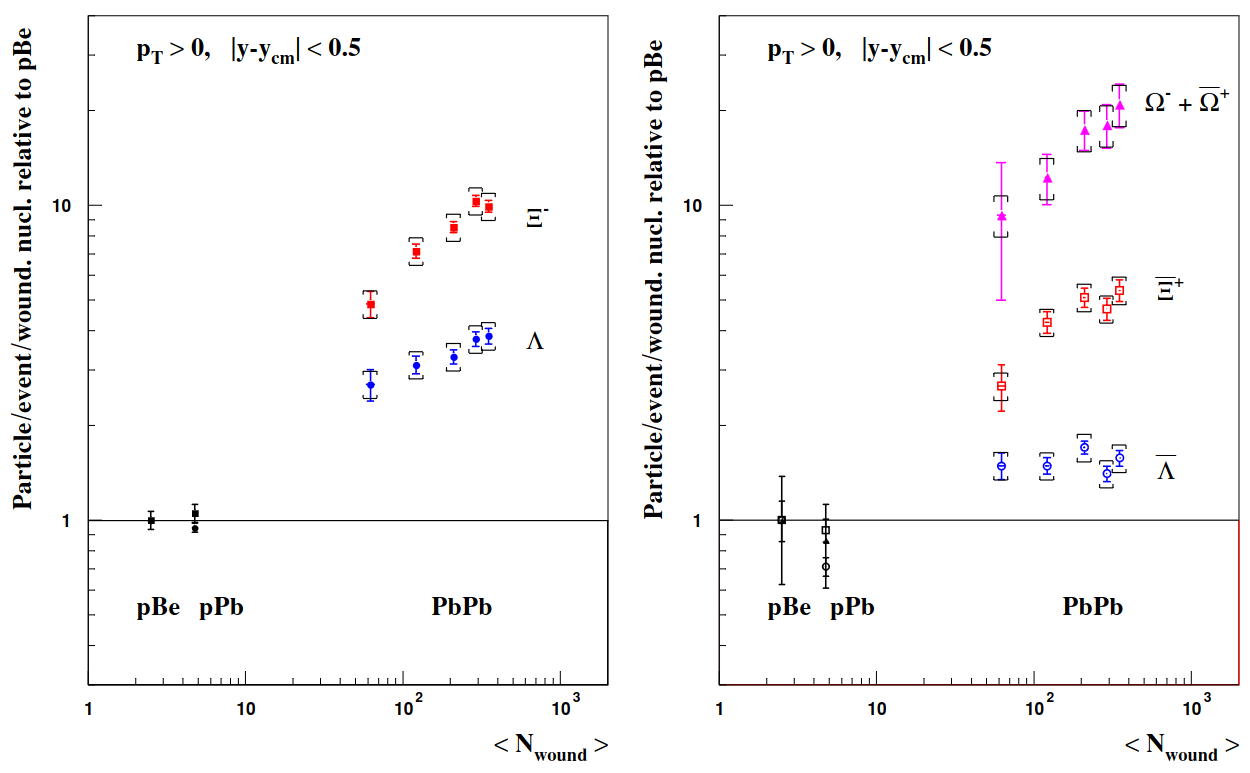
\includegraphics[width=1.0\textwidth]{strangeness-enhancement.png}};
      \node[font=\tiny] at (-0.5,2) {\textbf{Strangeness enhancement observed by NA57 at SPS (CERN)}};
      \node[font=\tiny] at (-1.6,-1.85) {\href{https://arxiv.org/abs/nucl-ex/0403016v2}{arXiv:nucl-ex/0403016}};
    \end{tikzpicture}

  \end{columns}


\end{frame}

     \begin{frame}
  \frametitle{\textbf{Charged Particle Suppression}}
  \begin{columns}
    \column{0.5\textwidth}
    \begin{itemize}
    \item Charged hadrons \textbf{heavily suppressed} in central collisions, but not in peripheral collisions
    \item Charged-hadron $R_{\text{AA}}$: measure of the suppression of charged hadrons in AA collisions as compared to pp collisions
    \end{itemize}
    \begin{align*}
      \boxed{R_{\text{AA}}^{\text{ch}} (p_{\text{T}}) = \cfrac{dN^{\text{AA}}_{\text{ch}} / dp_{\text{T}}}{\left< N_{\text{coll}} \right> dN^{\text{pp}}_{\text{ch}} / dp_{\text{T}}}}
    \end{align*}


    \begin{itemize}
    \item No suppression in small systems (pp, pPb)
    \item Colorless objects ($\gamma, W^{\pm}, Z$) are not suppressed
    \item Partons \textbf{lose energy via color interactions} as they traverse the QGP 
    \end{itemize}
    \column{0.5\textwidth}
    \begin{tikzpicture}
      \node{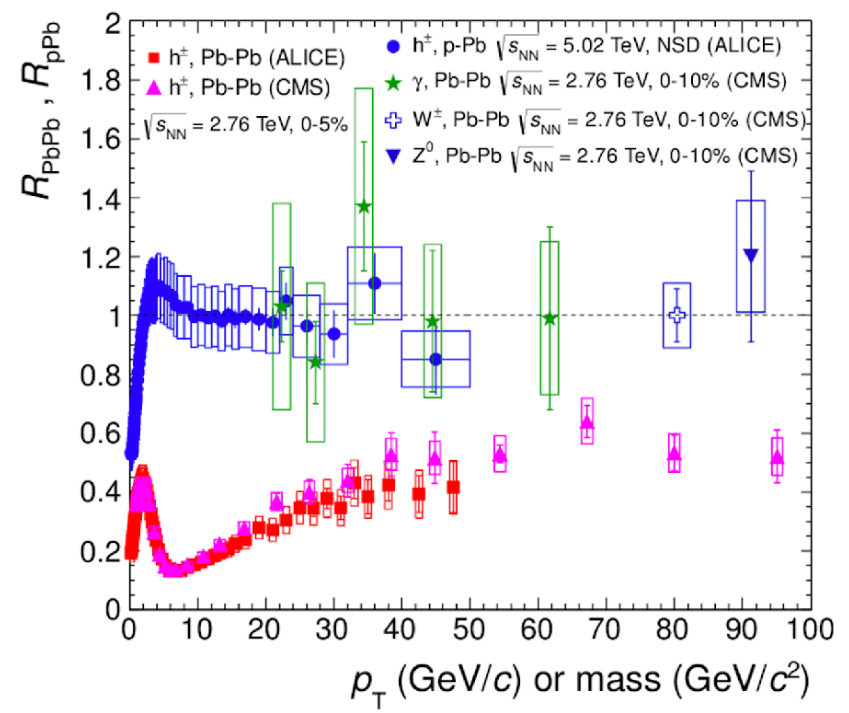
\includegraphics[width=\textwidth]{RAA-neutral-and-charged.png}};
      \node[font=\tiny] at (1.8,2.6) {\href{https://arxiv.org/abs/1012.1004}{arXiv:1012.1004}};
    \end{tikzpicture}
  \end{columns}
\end{frame}

     \begin{frame}
  \centering \textbf{Jets as Probes of the QGP}       
\end{frame}

     \begin{frame}
  \frametitle{\textbf{Hard processes in pp}}
  
  \begin{itemize}
  \item \textbf{Hard processes}: high-energy interaction between quarks and gluons
  \item Hard-process $\to$ \color{blue} short-distance physics \color{black} of partons $\bigotimes$ \color{red} long-distance phyiscs \color{black} of hadrons
  \end{itemize}

  \
  
  \centering Cross-section factorization in pp collisions
  \begin{align*}
    d\sigma^{p+p \to h + X} &= \sum_f \color{blue}d\sigma^{p+p \to f + X} \color{black}\bigotimes \color{red}D_{f \to h} (z, \mu^2) \\
    \color{black} &= \sum_{\color{blue}i,j,X\color{black},f,...}\color{blue} f_{i/p}(x_1,Q^2) \bigotimes f_{j/p}(x_2,Q^2) \bigotimes \hat{\sigma}_{ij\to f + X ...} \color{black}\bigotimes \color{red}D_{f \to h} (z, \mu^2)
  \end{align*}
  \begin{itemize}
  \item We use hard processes in pp collisions as a reference when we study QGP medium effects
  \end{itemize}
  \begin{columns}
    \column{0.6\textwidth}
    \centering
    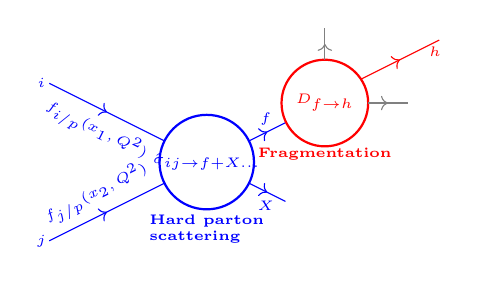
\begin{tikzpicture}
      \draw[-,blue,middlearrow={>}] (-2,1) to (-0.5366,0.2683);
      \draw[-,blue,middlearrow={>}] (-2,-1) to (-0.5366,-0.2683);
      \draw[blue,thick] (0,0) circle (0.6) node[font=\tiny]{$\hat{\sigma}_{ij\to f + X ...}$};
      \draw[-,blue,middlearrow={>}] (0.5366,0.2683) to (1,0.5);
      \draw[-,blue,middlearrow={>}] (0.5366,-0.2683) to (1,-0.5);
      %\draw[rotate=120,blue] (0,0) circle(0.5cm and 0.2cm);
      \draw[red,thick] (1.5,0.75) circle (0.55) node[font=\tiny]{$D_{f \to h}$};
      \draw[-,red,middlearrow={>}] (1.953,1.05) to (2.953,1.55);
      \draw[-,gray,middlearrow={>}] (1.5,1.3) to (1.5,1.7);
      \draw[-,gray,middlearrow={>}] (2.05,0.75) to (2.55,0.75);
      \node[font=\tiny,blue,align=left] at (0,-0.85) {\textbf{Hard parton} \\ \textbf{scattering}};
      \node[font=\tiny,red,align=left] at (1.5,0.1) {\textbf{Fragmentation}};
      \node[font=\tiny,blue,rotate=-26.56] at (-1.4,0.4) {$f_{i/p}(x_1,Q^2)$};
      \node[font=\tiny,blue,rotate=26.56] at (-1.4,-0.4) {$f_{j/p}(x_2,Q^2)$};
      \node[font=\tiny,red] at (2.9,1.4) {$h$};
      \node[font=\tiny,blue] at (-2.1,1) {$i$};
      \node[font=\tiny,blue] at (-2.1,-1) {$j$};
      \node[font=\tiny,blue] at (0.75,-0.55) {$X$};
      \node[font=\tiny,blue] at (0.75,0.55) {$f$};
    \end{tikzpicture}
    \column{0.4\textwidth}
    \begin{itemize}
    \item Cross-section in vacuum is perturbatively calculable!
    \item Fragmentation is non-perturbative $\to$ must rely on QCD-inspired models
    \item Leading hadron $\to$ \textbf{hard probe}
    \end{itemize}
  \end{columns}
  
\end{frame}

     \begin{frame}
  \frametitle{\textbf{Hard Processes in AA}}

  \begin{itemize}
  \item \textbf{Hard processes in AA}: high-energy interaction between quarks and gluons, followed by the production of QGP if system reaches sufficient energy density
  \item Hard-process time-scales $\to$ \color{blue} short-distance physics \color{black} of partons $\bigotimes$ \color{orange} energy loss \color{black} of partons in the QGP $\bigotimes$ \color{red} long-distance phyiscs \color{black} of hadrons
  \end{itemize}

  \
  
  \centering Cross-section factorization in AA collisions
  \begin{align*}
    d\sigma^{A+A \to h + X} &= \sum_f \color{blue}d\sigma^{A+A \to f + X}_{(\text{vac})} \color{black}\bigotimes \color{orange} P_f(\Delta E, L, \hat{q}) \color{black} \bigotimes \color{red}D^{\text{(vac)}}_{f \to h} (z, \mu^2) 
  \end{align*}
  \begin{columns}
    \column{0.6\textwidth}
    \centering
    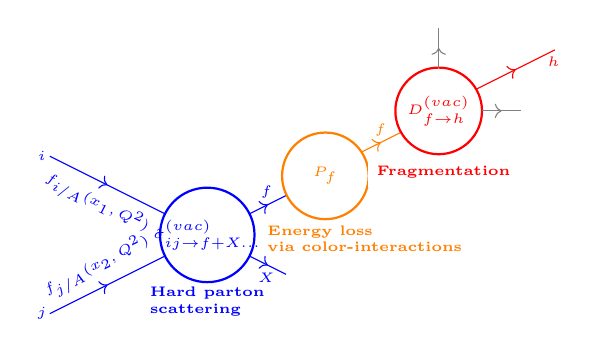
\begin{tikzpicture}
      \draw[-,blue,middlearrow={>}] (-2,1) to (-0.5366,0.2683);
      \draw[-,blue,middlearrow={>}] (-2,-1) to (-0.5366,-0.2683);
      \draw[blue,thick] (0,0) circle (0.6) node[font=\tiny]{$\hat{\sigma}_{ij\to f + X ...}^{\text{(vac)}}$};
      \draw[-,blue,middlearrow={>}] (0.5366,0.2683) to (1,0.5);
      \draw[-,blue,middlearrow={>}] (0.5366,-0.2683) to (1,-0.5);
      %\draw[rotate=120,blue] (0,0) circle(0.5cm and 0.2cm);
      \draw[orange,thick] (1.5,0.75) circle (0.55) node[font=\tiny]{$P_f$};
      \draw[-,orange,middlearrow={>}] (1.953,1.05) to (2.453,1.3);
      \node[font=\tiny,orange] at (2.2,1.33) {$f$};
      \node[font=\tiny,blue,align=left] at (0,-0.85) {\textbf{Hard parton} \\ \textbf{scattering}};
      \node[font=\tiny,orange,align=left] at (2,-0.05) {\textbf{Energy loss} \\ \textbf{via color-interactions}};
      \node[font=\tiny,blue,rotate=-26.56] at (-1.4,0.4) {$f_{i/A}(x_1,Q^2)$};
      \node[font=\tiny,blue,rotate=26.56] at (-1.4,-0.4) {$f_{j/A}(x_2,Q^2)$};
      \node[font=\tiny,blue] at (-2.1,1) {$i$};
      \node[font=\tiny,blue] at (-2.1,-1) {$j$};
      \node[font=\tiny,blue] at (0.75,-0.55) {$X$};
      \node[font=\tiny,blue] at (0.75,0.55) {$f$};
      \draw[red,thick] (2.939,1.575) circle (0.55) node[font=\tiny]{$D^{\text{(vac)}}_{f \to h}$};
      %\draw[orange,thick] (2.939,1.575) circle (0.58) ;
      \draw[-,red,middlearrow={>}] (3.415,1.85) to (4.415,2.35);
      \node[font=\tiny,red] at (4.4,2.2) {$h$};
      \draw[-,gray,middlearrow={>}] (2.939,2.125) to (2.939,2.625);
      \draw[-,gray,middlearrow={>}] (3.489,1.575) to (3.989,1.575);
      %\node[font=\tiny,gray] at (2.8,2.7) {X};
      %\node[font=\tiny,gray] at (4.2,1.57) {X};
      \node[font=\tiny,red,align=left,fill=white] at (3,0.80) {\textbf{Fragmentation}};
    \end{tikzpicture}
    \column{0.4\textwidth}
    \begin{itemize}
    \item Factorization theorems unkown for processes embedded in a QGP medium
    \item Vacuum-like hard-scattering and fragmentation
    \item How is energy transfered to the medium?
      \begin{itemize}
      \item Collisional energy loss
        \begin{itemize}
        \item Elastic scattering with medium, high $p$
        \end{itemize}
      \item Radiative energy loss
        \begin{itemize}
        \item Inelastic scattering with medium (gluon Bremsstrahlung), low $p$
        \end{itemize}
      \end{itemize}
    \end{itemize}
  \end{columns}
\end{frame}

     \begin{frame}
  \frametitle{\textbf{Jets}}
  \begin{columns}
    \column{0.5\textwidth}
    \begin{itemize}
    \item A jet is
      \begin{itemize}
      \item the result of a \textbf{high-}$\boldmath{Q^2}$ parton-parton interaction
      \item a \textbf{collimated spray of hadrons} resulting from parton fragmentation
      \item a \textbf{self-generating hard-probe} of the QGP
      \end{itemize}
    \item Jets are \textbf{well calibrated} in small systems (pp, $e^+ e^-$)
    \item Jets are often produced in back-to-back pairs
    \item $\tau^{\text{hard-scatter}} \ll \tau^{\text{QGP-formation}}$ $\to$ initial state unaffected by medium
    \item Use \textbf{relative jet yields} in pp and PbPb to measure medium properties
    \end{itemize}
    \column{0.5\textwidth}
    \centering 
    
    \begin{tikzpicture}
      \node{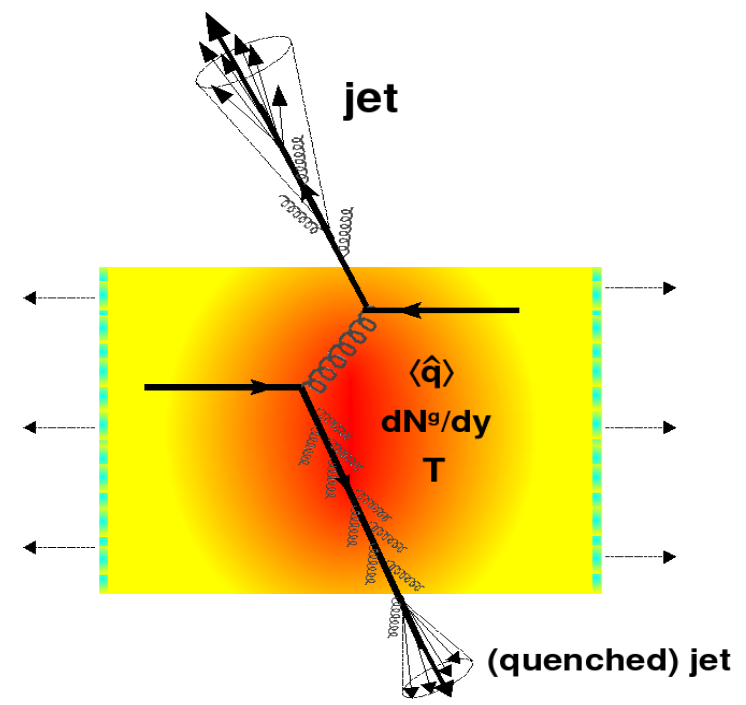
\includegraphics[width=0.8\textwidth]{jet-quenching.png}};
      \node[font=\tiny] at (1.5,1) {\href{https://arxiv.org/abs/0902.2011}{arXiv:0902.2011}};
    \end{tikzpicture}

    \

    \begin{tikzpicture}
      \node{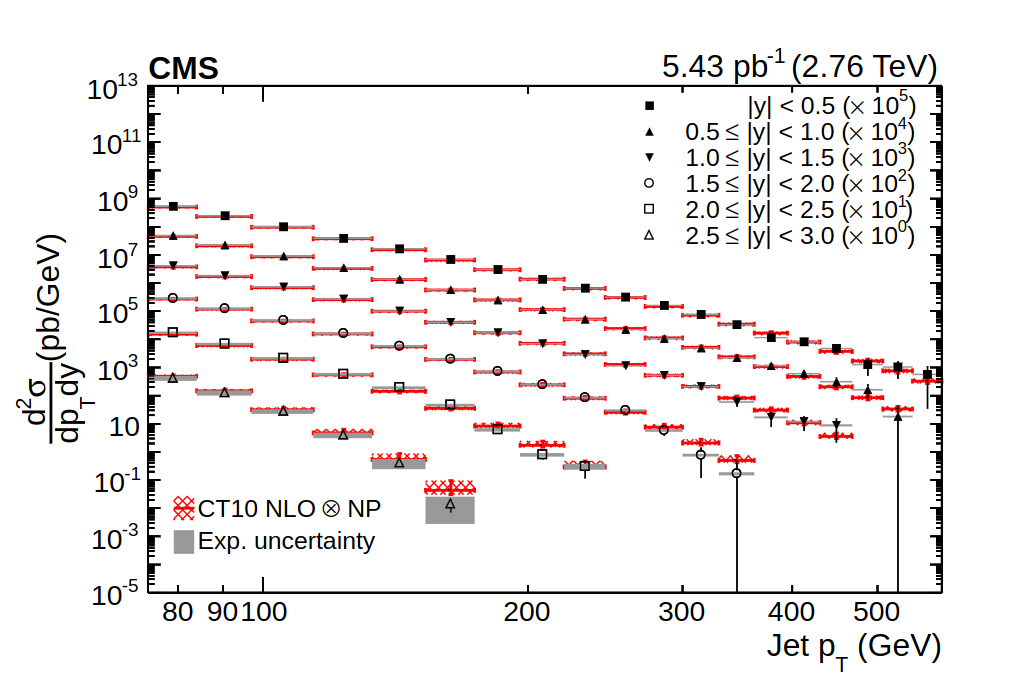
\includegraphics[width=0.8\textwidth]{jet-cross-section-data-vs-theory.png}};
      \node[font=\tiny] at (0.2,1.6) {\textbf{Jet production cross-section: data vs. theory}};
      \node[font=\tiny] at (-0.4,1.0) {\textbf{pp}};
      \node[font=\tiny] at (1.5,1) {\href{https://arxiv.org/abs/1512.06212}{arXiv:1512.06212}};
    \end{tikzpicture}


  \end{columns}







\end{frame}

     \begin{frame}
  \frametitle{\textbf{Jets in Experiment}}
  \begin{columns}
    \column{0.5\textwidth}
    \begin{itemize}
    \item A jet is the result of a \textbf{jet algorithm}, which is a computational process to cluster groups of collimated particles
    \item There are many types of jet algorithms, often differentiated by their choice of ``distance parameter''
    \end{itemize}
    \begin{align*}
      d_{ij} &= \min(p_{\text{T},i}^{2k},p_{\text{T},j}^{2k} )\cfrac{\Delta R_{ij}^2}{R^2} \\
      &k = 0 \to \text{Cambridge-Aachen algorithm} \\
        &k = 1 \to k_{\text{T}} \text{ algorithm} \\
          &k = -1 \to \text{anti-}k_{\text{T}} \text{ algorithm} \\
    \end{align*}
    \begin{itemize}
    \item Iteratively cluster pairs of tracks with smallest $d_{ij}$ and ``build'' jets
    \end{itemize}

    \column{0.5\textwidth}
    \centering
    \begin{tikzpicture}
      \node{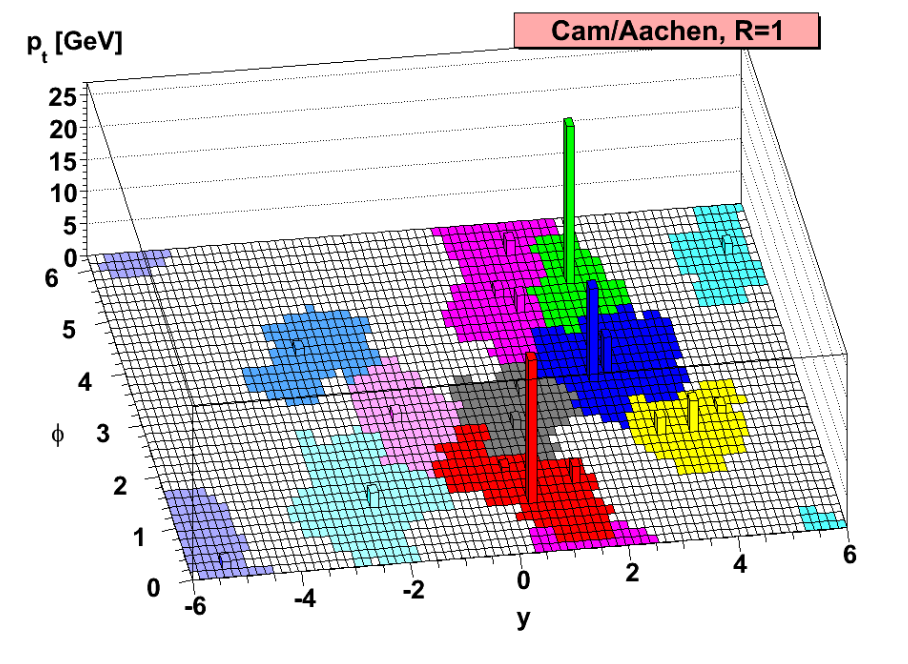
\includegraphics[width=0.6\textwidth]{cam-aachen.png}};
    \end{tikzpicture}

    \centering
    \begin{tikzpicture}
      \node{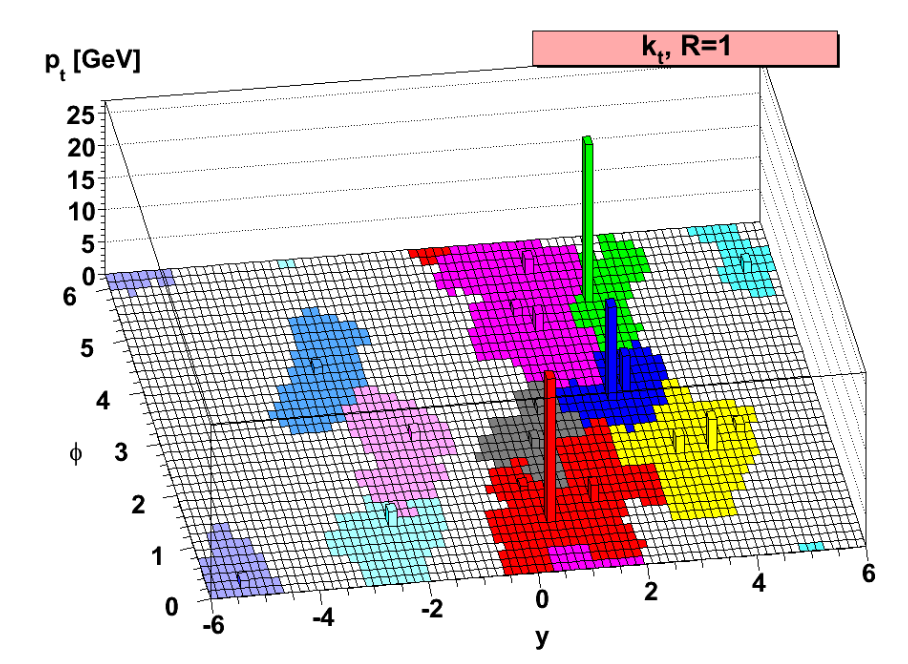
\includegraphics[width=0.6\textwidth]{kt.png}};
    \end{tikzpicture}

    \centering
    \begin{tikzpicture}
      \node{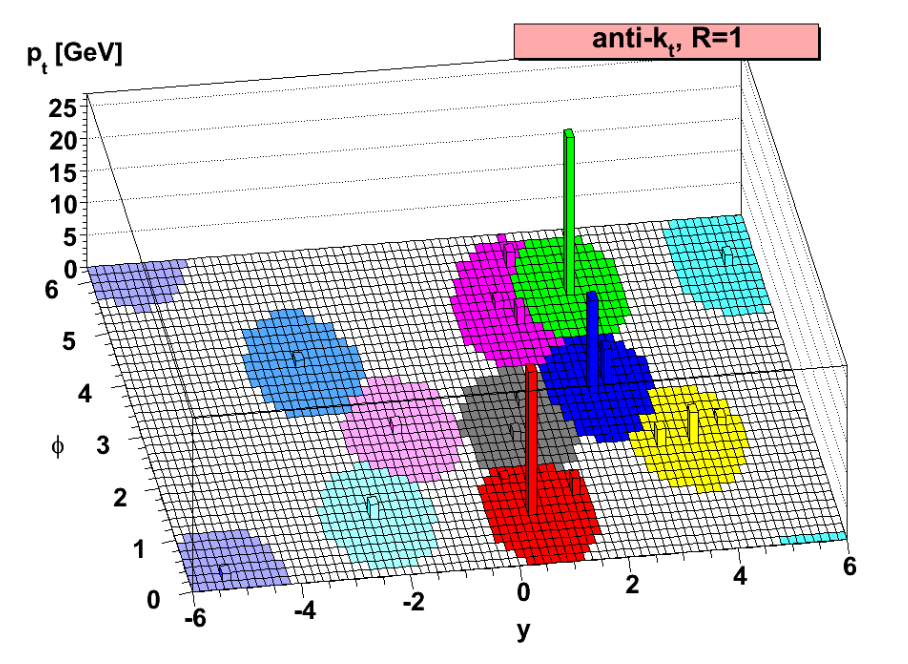
\includegraphics[width=0.6\textwidth]{anti-kt.png}};
    \end{tikzpicture}
  \end{columns}
\end{frame}

     \begin{frame}
  \frametitle{\textbf{Jet Suppression and Asymmetry}}
  \begin{columns}
    
    \column{0.5\textwidth}

    \begin{tikzpicture}
      \node{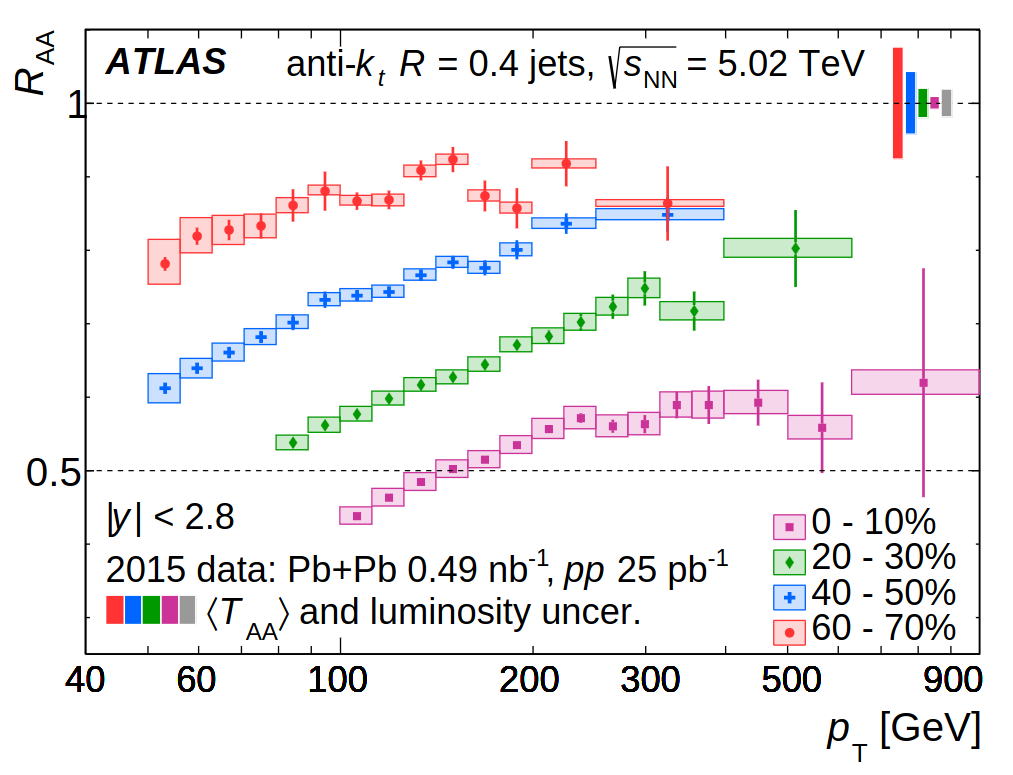
\includegraphics[width=\textwidth]{atlas-jet-raa.png}};
      \node[font=\tiny] at (-1,-2) {\href{https://arxiv.org/abs/1805.05635}{arXiv:1805.05635}};
    \end{tikzpicture}

    \

    
    \begin{tikzpicture}
      \node{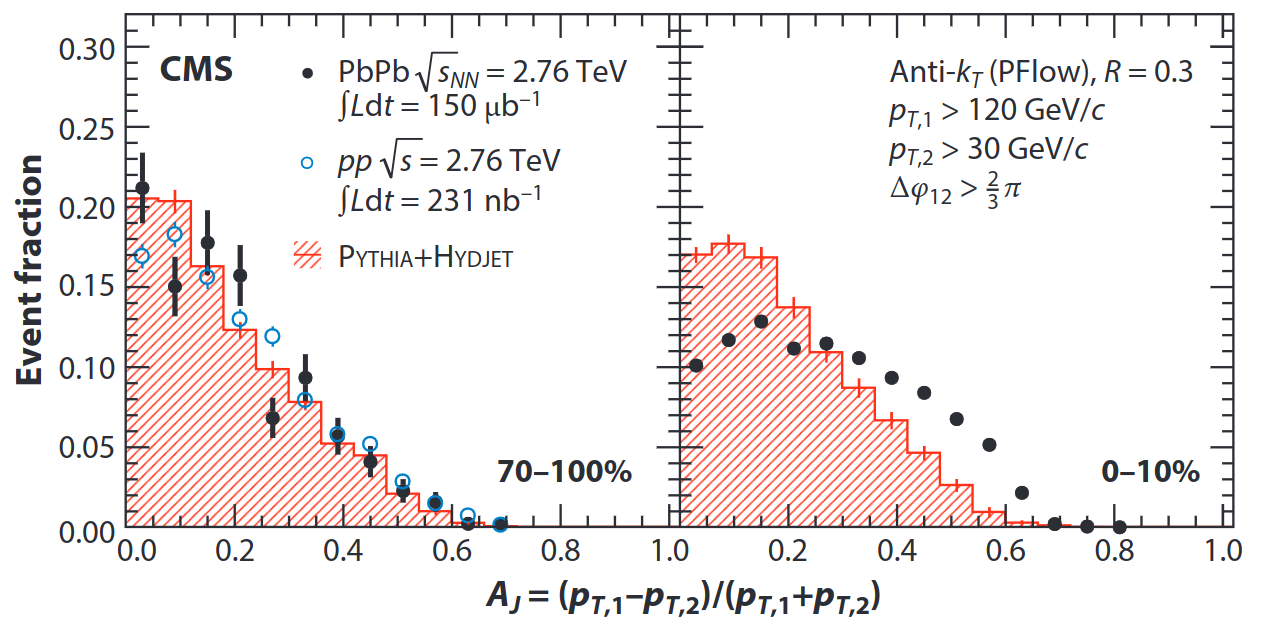
\includegraphics[width=\textwidth]{dijet-asymmetry.png}};
    \end{tikzpicture}

    \column{0.5\textwidth}
    \begin{itemize}
    %\item Fully-reconstructed jets are better probes of medium properties than leading hadrons
    \item Jet $R_{\text{AA}}$: measure of the suppression of jet production in AA collisions as compared to pp collisions
    %\item Fragmenting daughter-partons lose energy via gluon interactions $\to$ lose energy $\to$ final-state jet is ``suppressed''
    \end{itemize}
    \begin{align*}
      R_{\text{AA}}^{\text{jet}} (p_{\text{T}}) = \cfrac{dN^{\text{AA}}_{\text{jet}} / dp_{\text{T}}}{\left< N_{\text{coll}} \right> dN^{\text{pp}}_{\text{jet}} / dp_{\text{T}}}
    \end{align*}
    \begin{itemize}
    \item We expect asymmetric suppression in dijet events, since one jet will interact with more QGP than the other
    \item Quantify via dijet-asymmetry $A_J$
      \begin{align*}
        A_J = \cfrac{p_{\text{T},1} - p_{\text{T},2}}{p_{\text{T},1} + p_{\text{T},2}}
      \end{align*}
    \item Jet suppression \& asymmetry $\to$ \textbf{consistent with presence of QGP}
    \item Not seen in small systems (pp, pPb)
    \end{itemize}
  \end{columns}

\end{frame}

     \begin{frame}

  \frametitle{\textbf{Jet Shapes in HI Collisions}}

  \begin{columns}

    \column{0.4\textwidth}
    \begin{itemize}
    \item The \textbf{jet shape} is the transverse momentum weighted distribution of particles around the jet axis
    \end{itemize}
    \begin{align*}
      \rho(\Delta r) = \cfrac{1}{\delta r} \cfrac{1}{N_{\text{jets}}} \sum_{\text{jets}} \cfrac{\sum_{\text{tracks} \in [r_a, r_b)} p_{\text{T}}^{\text{ch}}}{p_{\text{T}}^{\text{jet}}}
    \end{align*}
    \begin{itemize}
    \item Jets are \textbf{broader} in central collisions
    \item Consistent with picture of a medium-modified parton cascade
    \item Energy is ``pushed out'' of the sides of the jet cone via broadening
    \end{itemize}
    
    \column{0.6\textwidth}

    \centering

    \begin{tikzpicture}
      \node{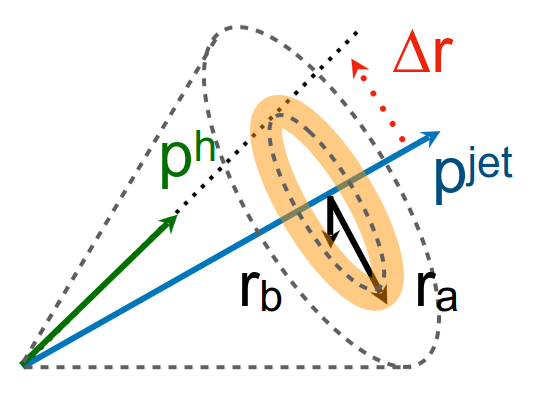
\includegraphics[width=0.5\textwidth]{jet-shape-cartoon.png}};
      \node[font=\tiny] at (1.5,1.6) {\href{https://indico.cern.ch/event/838105/contributions/3519117/attachments/1891832/3120100/HIN-18-020-approval.pdf}{HIN-18-020}};
    \end{tikzpicture}

    \

    \begin{tikzpicture}
      \node{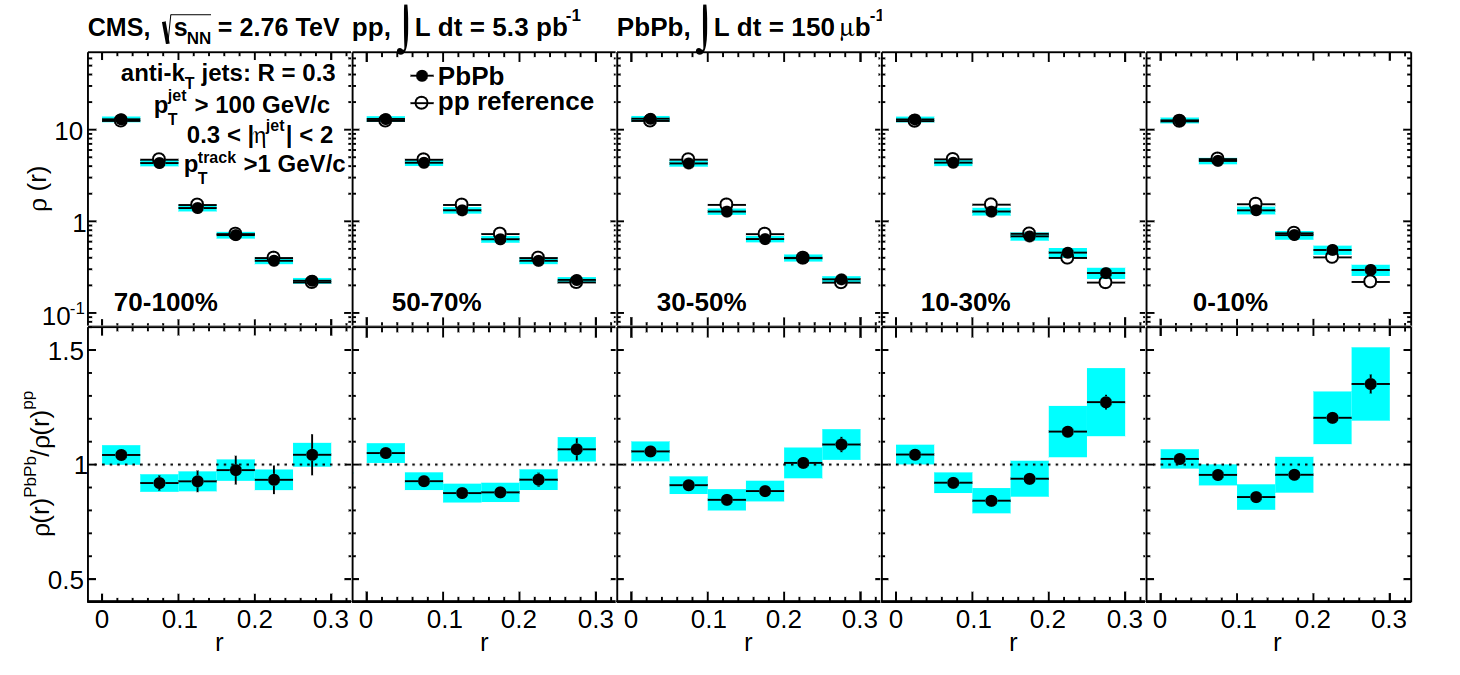
\includegraphics[width=\textwidth]{cms-jet-shape.png}};
      \node[font=\tiny] at (2,1.6) {\href{https://arxiv.org/abs/1102.1957}{arXiv:1102.1957}};
    \end{tikzpicture}


    
    

  \end{columns}






\end{frame}

     \begin{frame}
  \frametitle{\textbf{Jet Fragmentation in HI Collisions}}
  \begin{columns}
    \column{0.5\textwidth}
    \begin{tikzpicture}
      \node{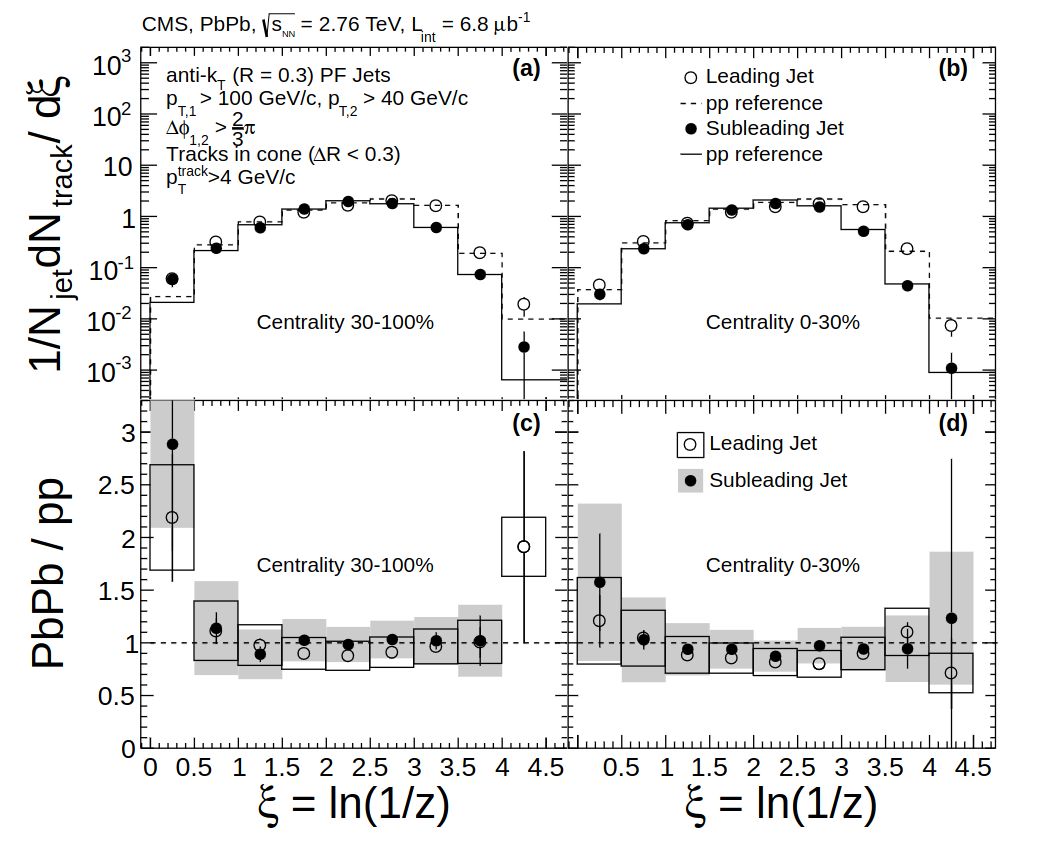
\includegraphics[width=\textwidth]{cms-fragmentation.png}};
    \end{tikzpicture}
    \column{0.5\textwidth}
    \begin{itemize}
    \item Parametrize in-jet energy distribution via variables $\xi$ and $z$
    \end{itemize}
    \begin{align*}
      \xi = \ln\frac{1}{z} ,\ \  z = \cfrac{p_\parallel^{\text{track}}}{p^{\text{jet}}}
    \end{align*}
    \begin{itemize}
    \item Fragmentation functions in PbPb consistent with pp $\to$ fragmentation is vacuum-like
    \item Partons lose energy prior \textbf{prior to fragmentation}, then redistribute their remaining energy as they would in vacuum
    \end{itemize}
  \end{columns}
\end{frame}

     \begin{frame}
  \frametitle{\textbf{Jet Flavor}}
  \begin{itemize}
  \item In MC, we know the jet's initial fragmenting parton $\to$ \textbf{jet flavor}
  \item \textit{Quark jets}: jets resulting from fragmenting $u$,$d$,$s$,$c$,$b$ quarks
  \item \textit{Gluon jets}: jets resulting from $g$ fragmentation
    \begin{itemize}
    \item Higher mulitplicity due to gluon self-splitting
    \end{itemize}
  \item In data, we cannot know the jet-flavor directly $\to$ must infer from other observables
  \end{itemize}

  \

  \begin{columns}
    \column{0.5\textwidth}
    \begin{tikzpicture}
      \node{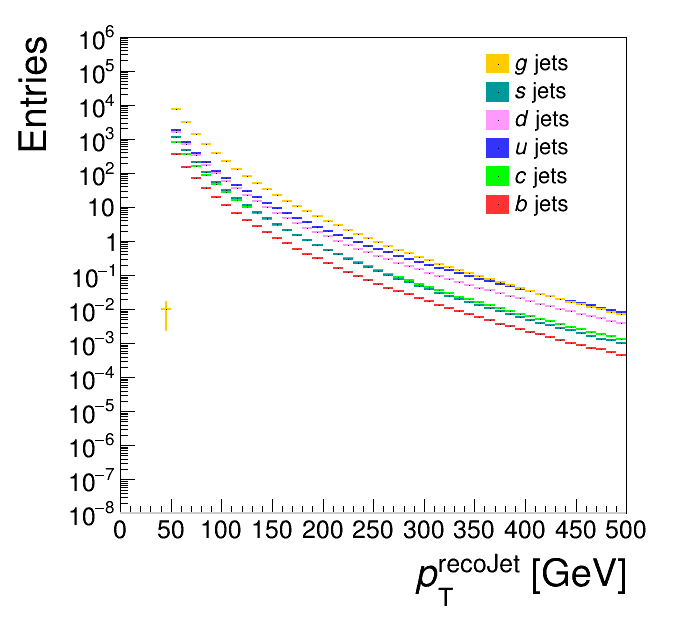
\includegraphics[width=0.8\textwidth]{flavor-spectra.png}};
    \end{tikzpicture}
    \column{0.5\textwidth}
    \begin{tikzpicture}
      \node{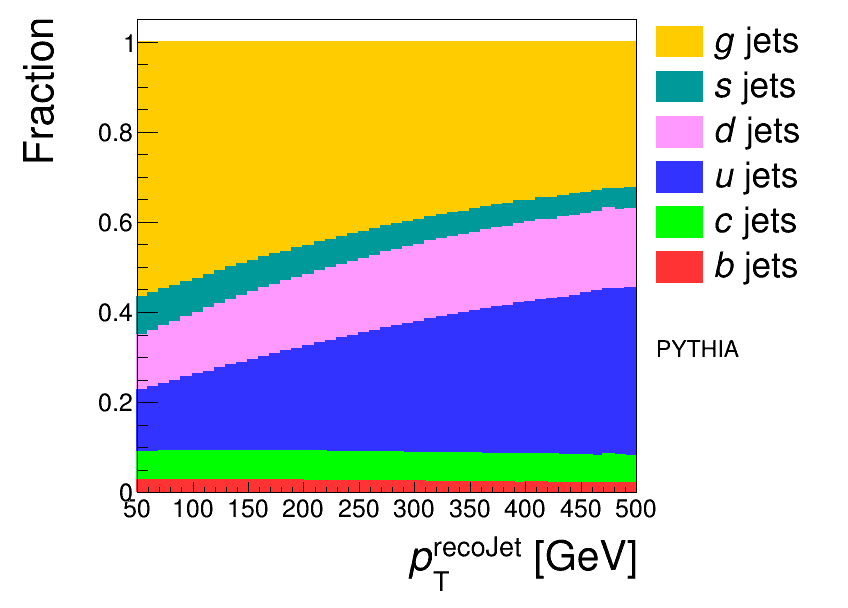
\includegraphics[width=1.0\textwidth]{flavor-fraction.png}};
    \end{tikzpicture}
  \end{columns}
\end{frame}

     \begin{frame}
  \centering
  $\boldmath{b}$\textbf{-jet measurements with CMS}
\end{frame}

     \begin{frame}
  \frametitle{\textbf{CMS Detector}}
  \centering \begin{tikzpicture}
    \node{\includegraphics[width=0.9\textwidth]{cms-detector.png}};
    \node[font=\tiny] at (4,3.5) {\href{https://arxiv.org/abs/1706.04965}{arXiv:1706.04965}};
  \end{tikzpicture}
\end{frame}

     \begin{frame}
  \frametitle{\textbf{CMS Detector}}
  \centering \begin{tikzpicture}
    \node{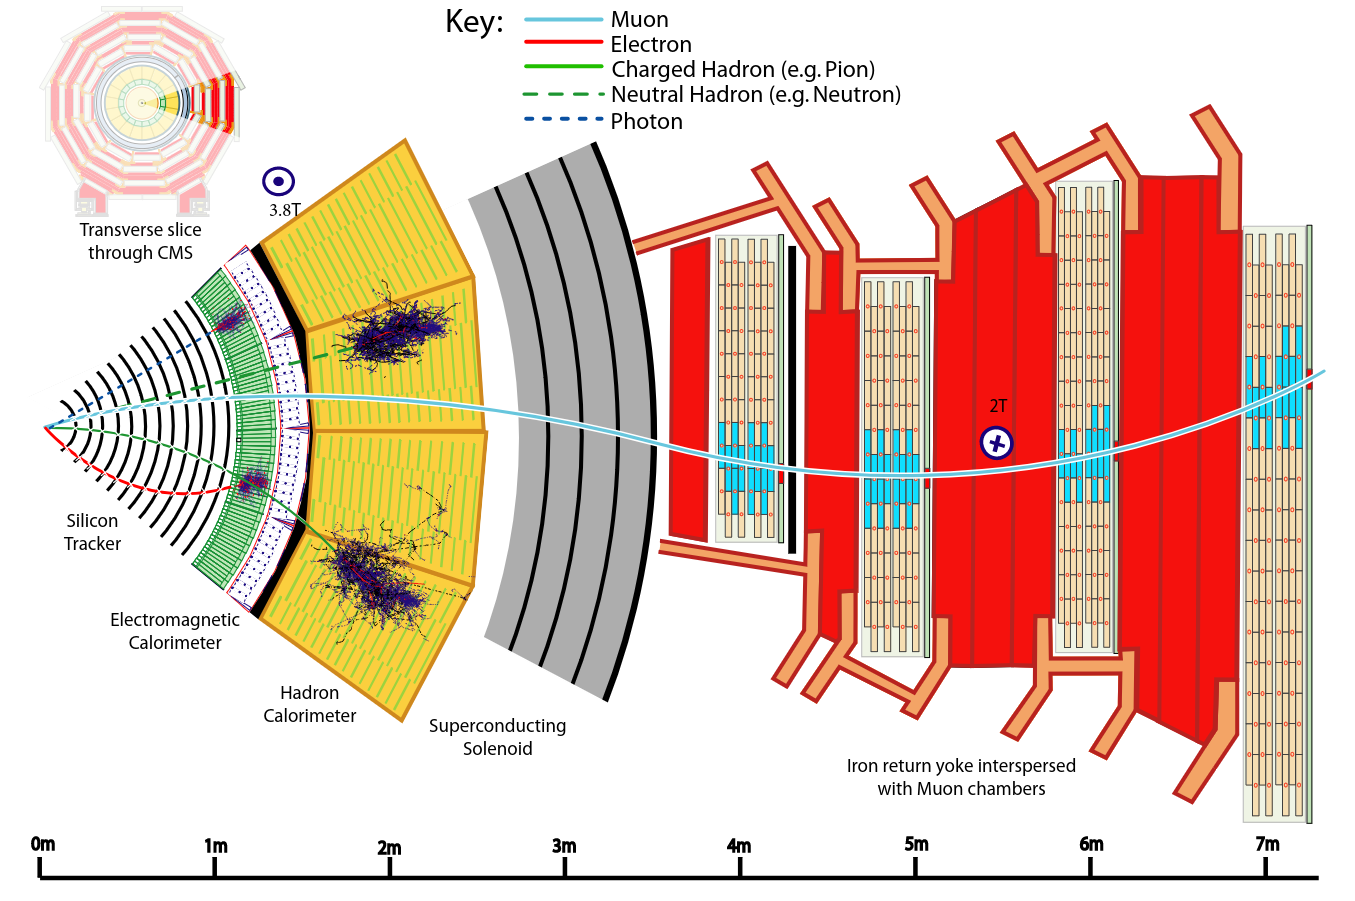
\includegraphics[width=0.9\textwidth]{cms-detector-slice.png}};
    \node[font=\tiny] at (4,3.5) {\href{https://arxiv.org/abs/1706.04965}{arXiv:1706.04965}};
  \end{tikzpicture}
\end{frame}

     \begin{frame}
  \frametitle{\textbf{$b$-jet Indetification}}
  \begin{columns}
    \column{0.5\textwidth}
    \begin{itemize}
    \item Many reconstructed objects can be used to discriminate between $b$ and light-jets
      \begin{itemize}
      \item Tracks
      \item Vertices
      \item Leptons
      \end{itemize}
    \item 3D impact paramater (IP)
      \begin{itemize}
      \item Track's distance-of-closest-approach to jet-axis
      \item Positive values: particle travelling along jet-axis
      \item $b$-quarks tend to have large IP because of longer lifetime
      \end{itemize}
    \item Combined-secondary-vertex (CSV) discriminator
      \begin{itemize}
      \item Combines vertex (and secondary vertex) information with track-based lifetime info in a complicated algorithm
      \item $b$-jets tend to contain secondary vertices
      \end{itemize}
    \item \textbf{Muon rel-}$\boldmath{p_{\text{T}}}$
      \begin{itemize}
      \item Measures muon's transverse momentum relative to jet-axis
      \item $b$-quarks tend to impart more transverse momentum into daughter muons
      \end{itemize}
    \end{itemize}
    \column{0.5\textwidth}
    \centering
    \begin{tikzpicture}
      \node{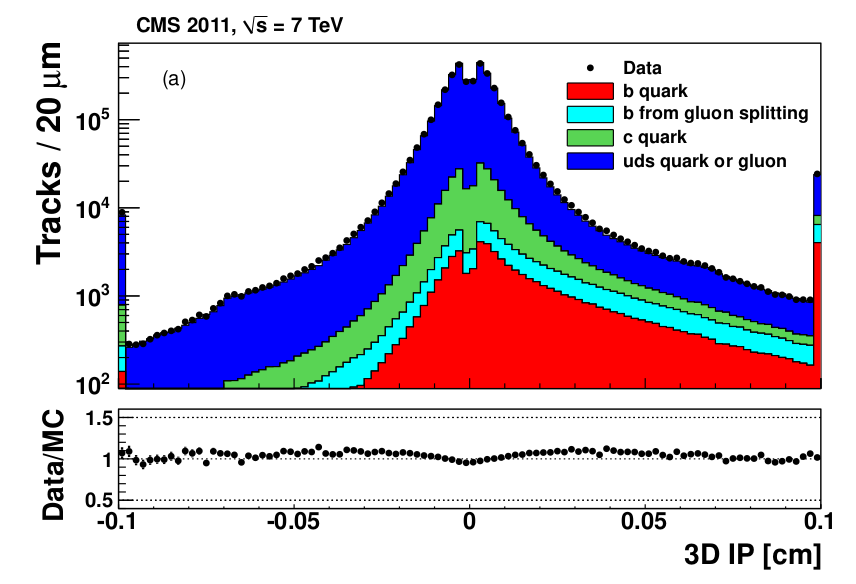
\includegraphics[width=0.58\textwidth]{b-IP.png}};
    \end{tikzpicture}
    \begin{tikzpicture}
      \node{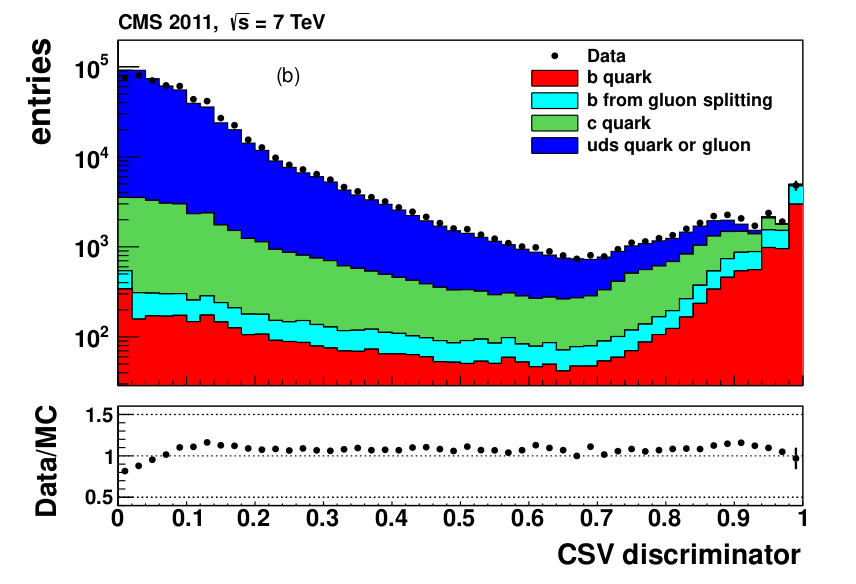
\includegraphics[width=0.58\textwidth]{csv-discriminator.png}};
    \end{tikzpicture}
    \begin{tikzpicture}
      \node{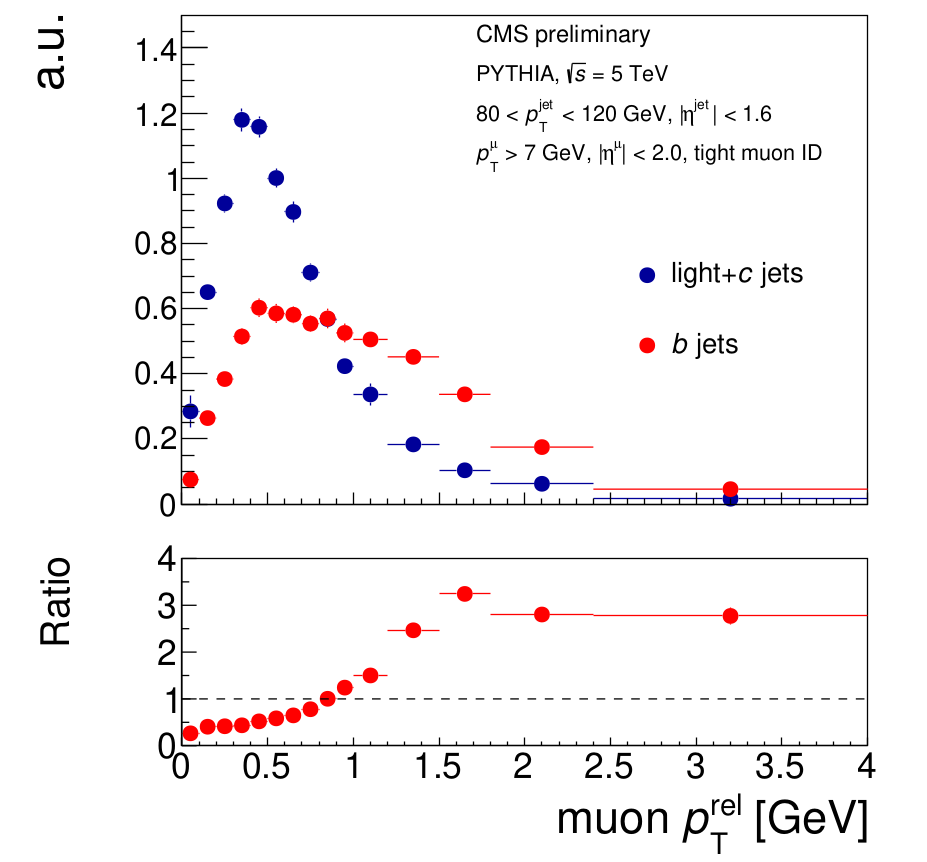
\includegraphics[width=0.58\textwidth]{muon-rel-pt.png}};
    \end{tikzpicture}
  \end{columns}
\end{frame}

     \begin{frame}

  \frametitle{\textbf{Muon-tagged Jets}}

  \begin{columns}
    \centering
    \column{0.5\textwidth}
    \begin{itemize}
    \item Muon-tagged jets are well described by data
    \item $\mu$-tagged $b$ and $c$-jets are under-reconstructed $\to$ neutrino production
    \end{itemize}
    \column{0.5\textwidth}
    \begin{tikzpicture}
      \node{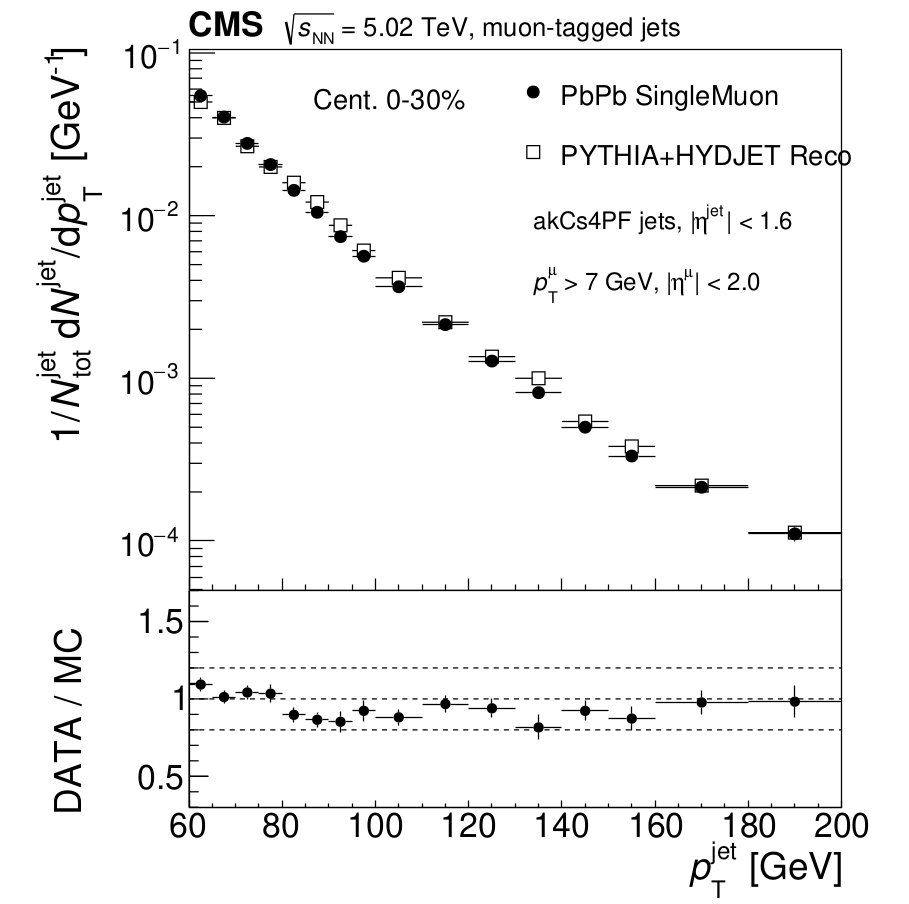
\includegraphics[width=0.6\textwidth]{muon-tagged-jet-spectra.png}};
    \end{tikzpicture}
  \end{columns}

  \begin{columns}
    \centering
    \column{0.75\textwidth}
    \begin{tikzpicture}
      \node{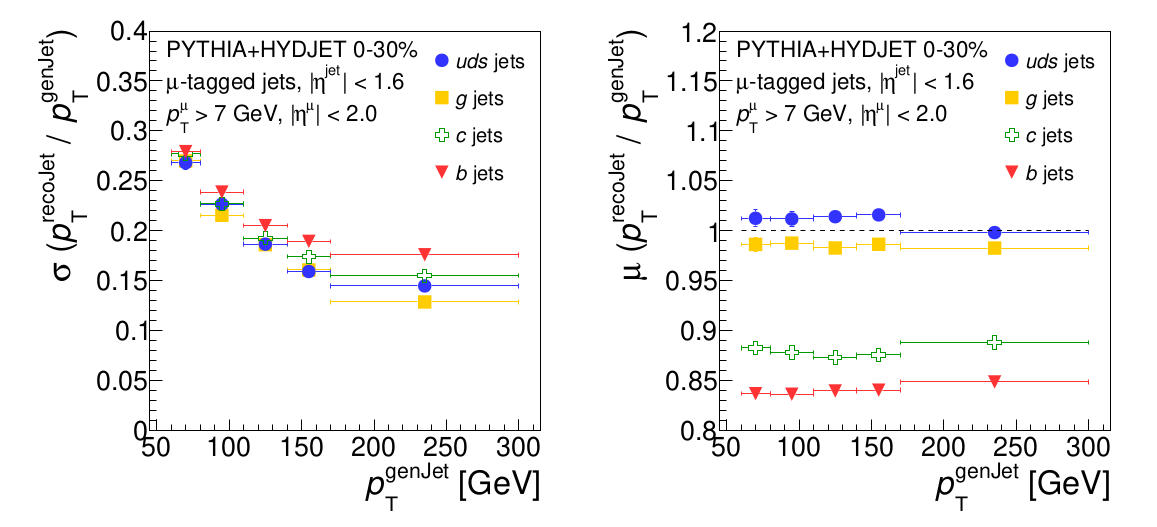
\includegraphics[width=1.0\textwidth]{JER-JES.png}};
    \end{tikzpicture}
  \end{columns}





\end{frame}

     \begin{frame}
  \frametitle{\textbf{Muon rel-}$\boldmath{p_{\text{T}}}$\textbf{ Template Fitting}}
  \begin{columns}
    \column{0.33\textwidth}
    \begin{tikzpicture}
      \node{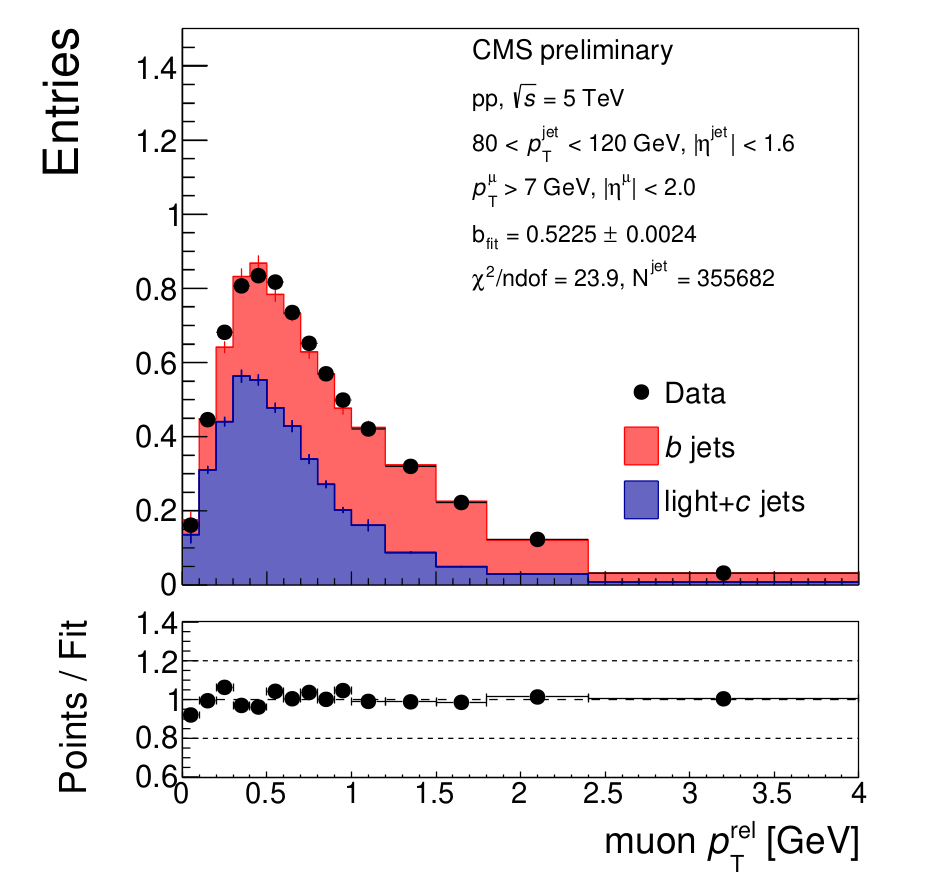
\includegraphics[width=\textwidth]{template-fit-pp.png}};
    \end{tikzpicture}
    \column{0.33\textwidth}
    \begin{tikzpicture}
      \node{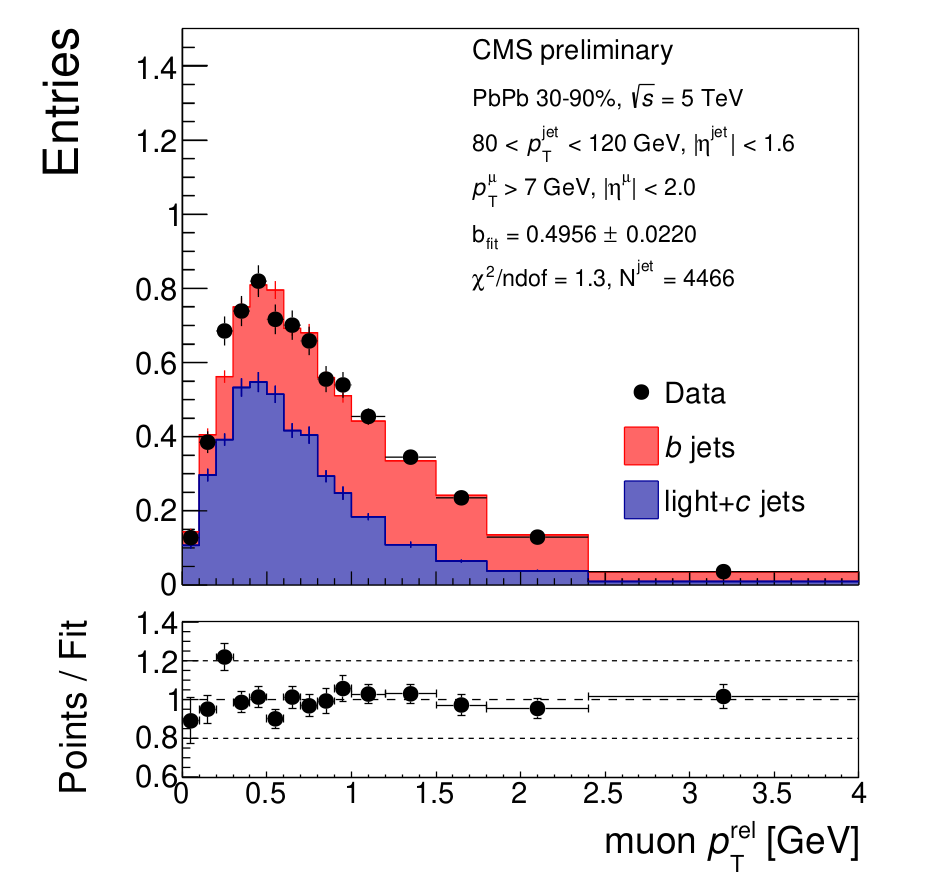
\includegraphics[width=\textwidth]{template-fit-PbPb-30-90.png}};
    \end{tikzpicture}
    \column{0.33\textwidth}
    \begin{tikzpicture}
      \node{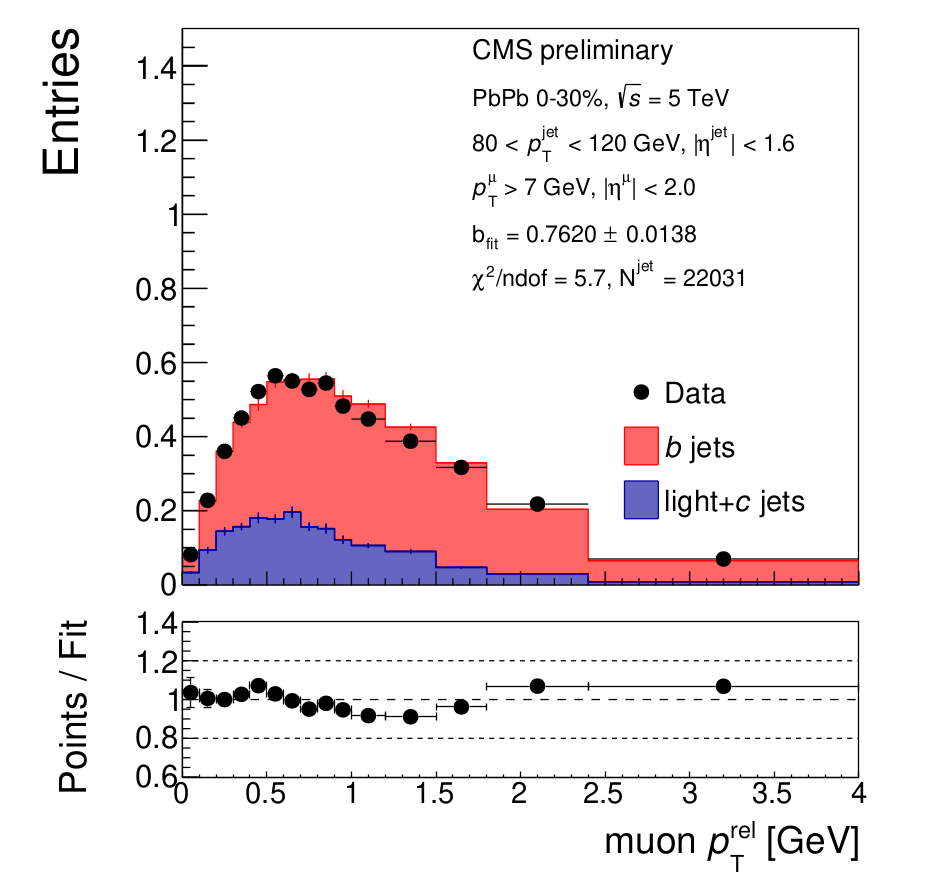
\includegraphics[width=\textwidth]{template-fit-PbPb-0-30.png}};
    \end{tikzpicture}
  \end{columns}

  \begin{columns}
    \column{0.33\textwidth}
    \begin{tikzpicture}
      \node{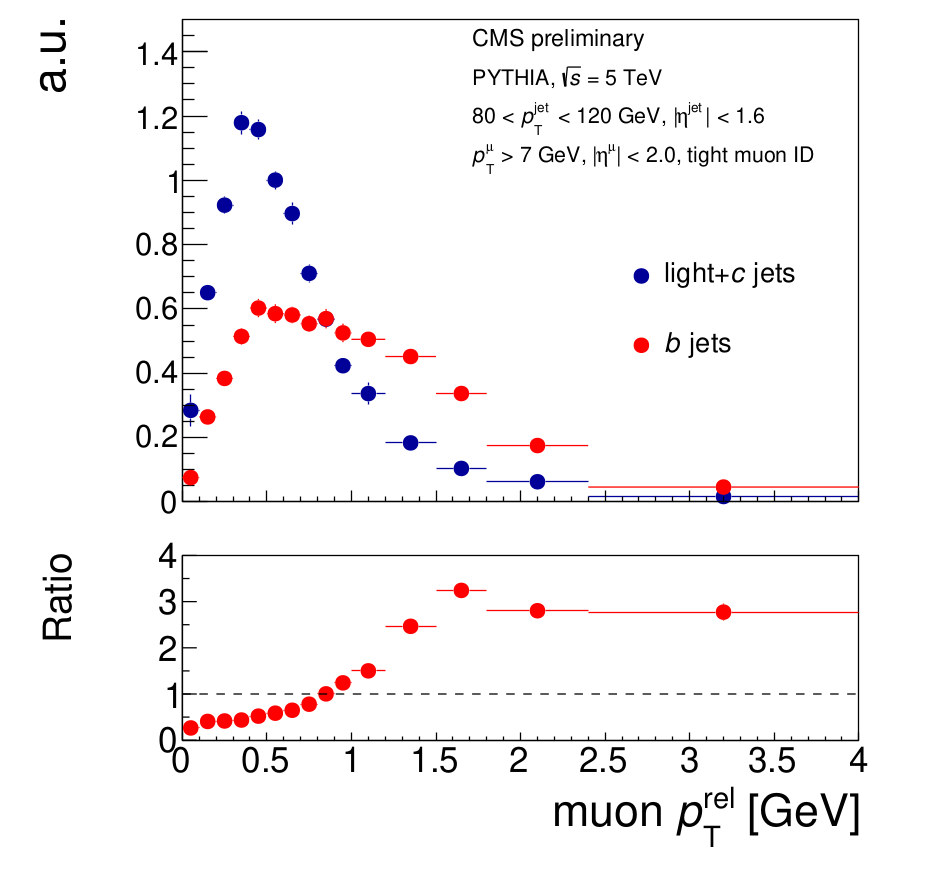
\includegraphics[width=\textwidth]{template-shape-pp.png}};
    \end{tikzpicture}
    \column{0.33\textwidth}
    \begin{tikzpicture}
      \node{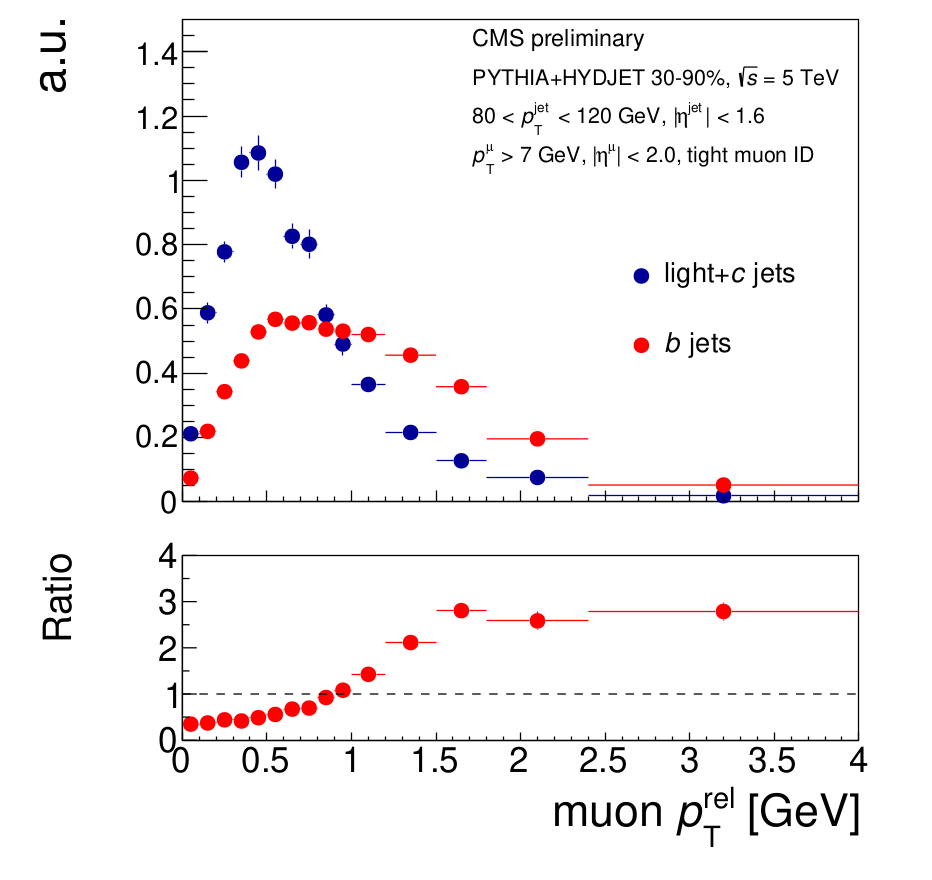
\includegraphics[width=\textwidth]{template-shape-PbPb-30-90.png}};
    \end{tikzpicture}
    \column{0.33\textwidth}
    \begin{tikzpicture}
      \node{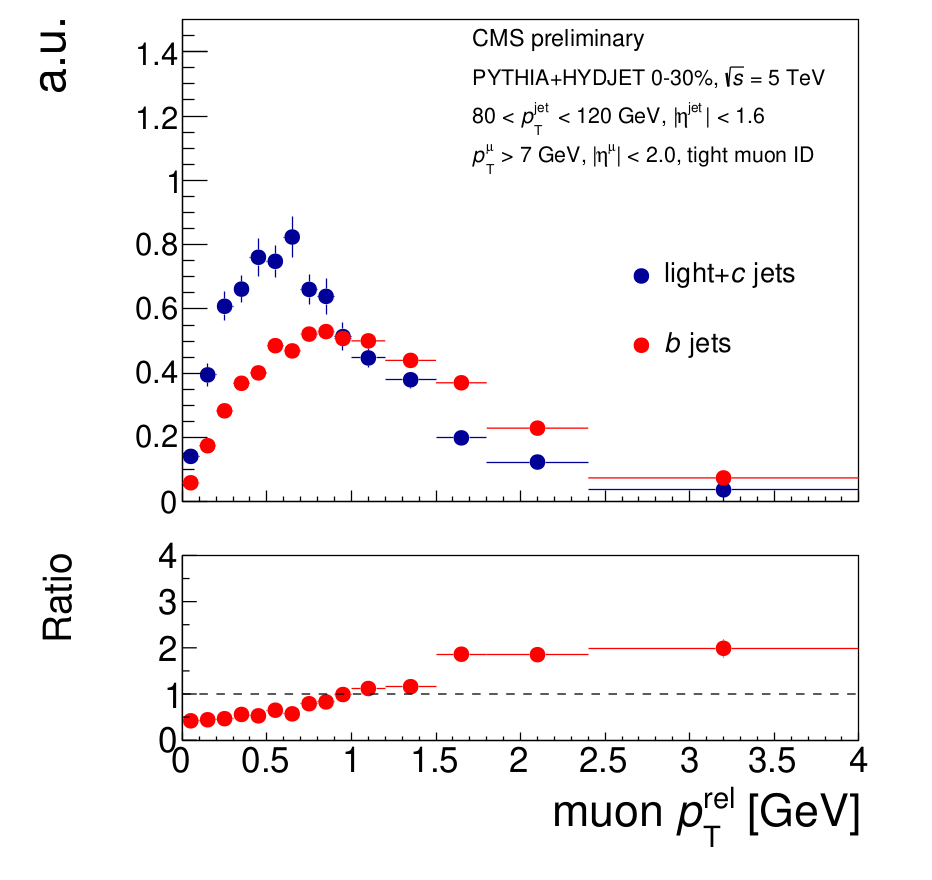
\includegraphics[width=\textwidth]{template-shape-PbPb-0-30.png}};
    \end{tikzpicture}
  \end{columns}



\end{frame}

     \begin{frame}
  \frametitle{\textbf{$b$-jet Purity and Fraction}}
  \begin{columns}
    \column{0.5\textwidth}
    \begin{itemize}
    \item $b$-purity measurements from template fits give us an estimated $b$-jet spectra
    \item Correct for trigger, muon-reconstruction, and matching efficiency
    \item Obtain an inclusive $b$-jet fraction
    \item Differences in inclusive $b$-jet fraction could indicate mass dependence on jet-quenching
    \item Work ongoing!
    \end{itemize}
    \column{0.5\textwidth}
    \centering
    \begin{tikzpicture}
      \node{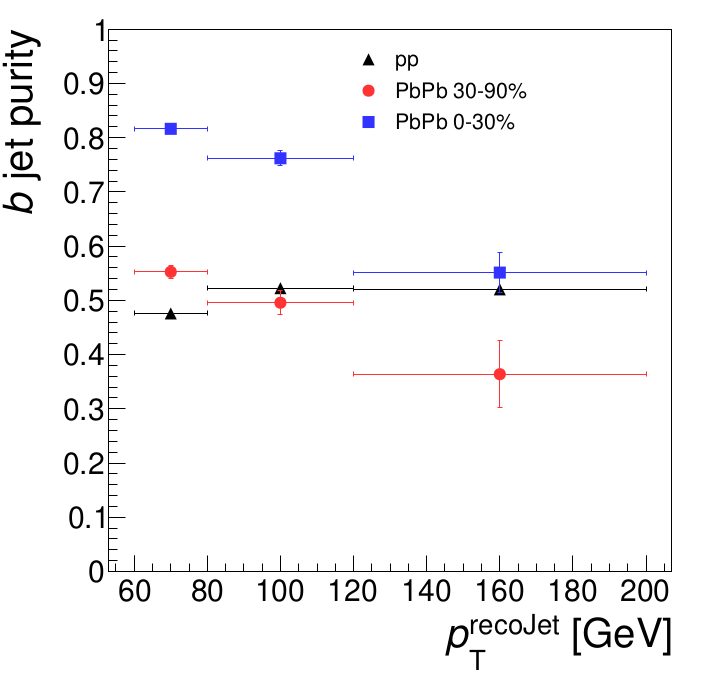
\includegraphics[width=0.7\textwidth]{b-purity.png}};
    \end{tikzpicture}

    \

    \begin{tikzpicture}
      \node{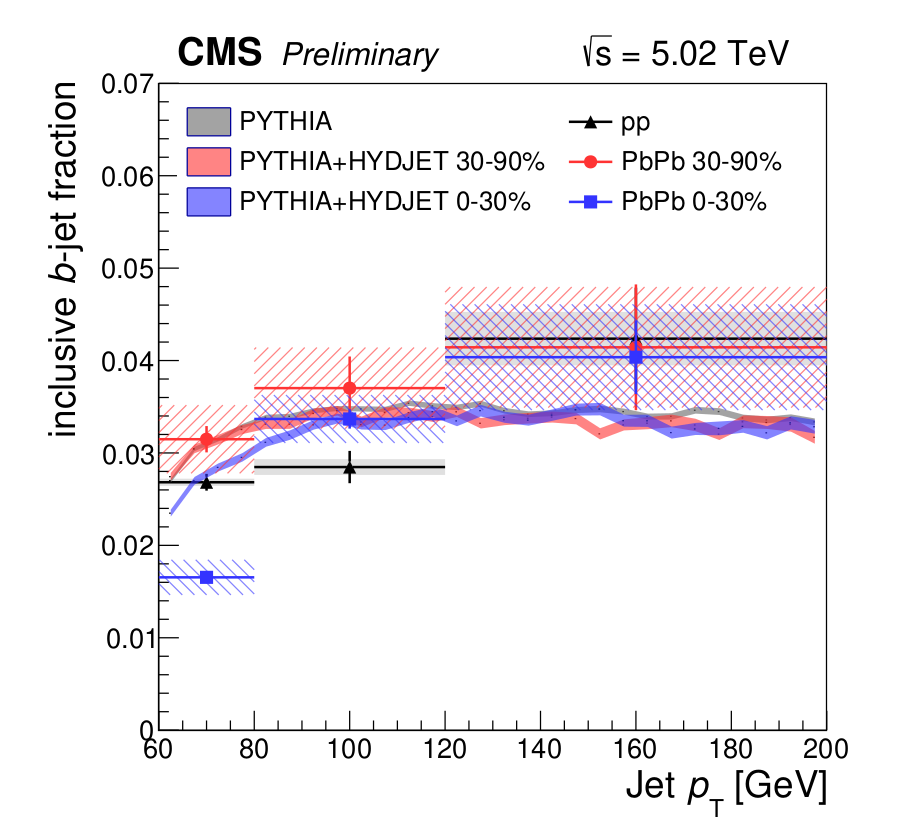
\includegraphics[width=0.7\textwidth]{b-fraction.png}};
    \end{tikzpicture}
    
  \end{columns}


\end{frame}

     \begin{frame}
\centering
\textbf{THANK YOU!}
\end{frame}











     




     \end{document}
